%!TEX root = bioPrediction_main.tex
%%!TEX root = bioPrediction_main.tex
%%!TEX root = bioPrediction_main.tex
%%!TEX root = bioPrediction_main.tex
%\input{bp_results_1}
%%\input{bp_results_2}

%\section{Analysis and Results}

%% To evaluate the efficacy of continuously predicting a knowledge worker's stress, focus, and awakeness in the workplace, we trained and tested machine learning classifiers using a leave-one-out cross validation. For prediction, we used the features extracted from the collected data as the input data, and binarized the participants' self-reported responses on stress, focus, and awakeness into two classes each (e.g., 'stressed' and 'not stressed') to use as output measures.

\section{Observed Trends Over Time in Stress and Awakeness Levels}
\label{stressTrends}

To gain insights into how knowledge workers experience stress and awakeness over an
extended period of work, we examined the end of day survey responses
collected from each participant to see if any identifiable trends
emerged. As we noted in the last section, we did not ask
participants about focus in the end of  day surveys as focus is an 
aspect relevant at a particular moment in time rather than an aspect
for an extended period of work. We used data from 13 of the 14 participants - we excluded one participant
from this analysis as they experienced atypical stress
levels in the latter half of the study due to factors outside of our
control.

\subsection{Stress Levels}
Overall, we identified three prominent characteristics in the stress levels.
%\rev{We describe characteristics noted in the reporting of the knowledge workers about the stress they experienced over the duration of the study.}

\begin{figure}[h!]
  \centering
      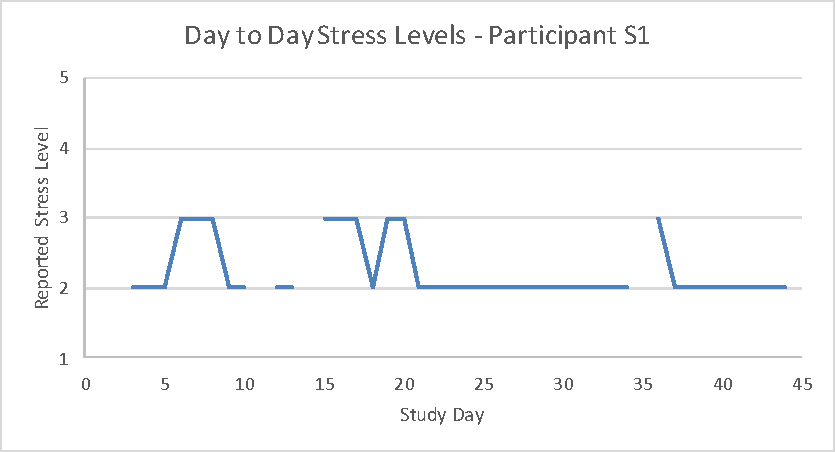
\includegraphics[width=0.7\textwidth]{s1_stress.pdf}
      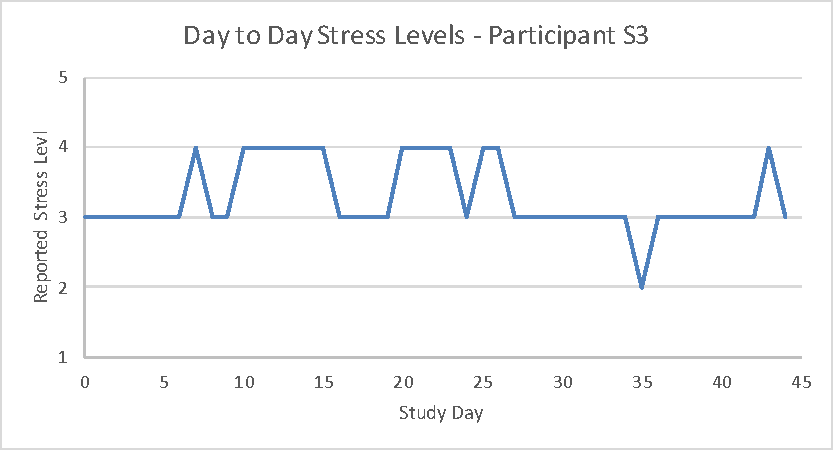
\includegraphics[width=0.7\textwidth]{s3_stress.pdf}
  \caption{The day-to-day stress levels reported by two participants (S1 and S3) are shown. The y-axis represents values on the 5-point Likert scale we asked participants to respond with ranging from 1/Not at all stressed to 5/Extremely stressed. The x-axis represents the day of the study on which the value was recorded (from 0-45). Some gaps are present in the chart for S1 as they did not report their stress level on those days.}
   \vspace*{-2mm}
   \label{fig:dailyStress}
\end{figure}


\subsubsection{Baseline Stress Levels}
%\noindent\textit{\textbf{Baseline Stress Levels.}}
Common amongst all participants was a trend to select one stress rating
far more frequently than any other. We will refer to this value as the
participant's baseline stress level. All but one participant reported
their perceived stress level for the day as their baseline stress
level more than 50\% of the time. In total, the baseline values made
up 65\% of the reported values collected from
participants. Interestingly, while participants sometimes saw periods
of sustained increases in stress, lasting as many as 6 consecutive
workdays in the most extreme case, participants would always return to
their baseline stress level at some point.


The baseline stress level varied significantly between participants. \rev{Seven}
participants (54\%) reported feeling average stress levels most frequently
(rating 3 on our scale), while \rev{five} (38\%) reported feeling little stress
(rating 2) and \rev{one} (8\%) reported feeling no stress at all (rating 1). Figure \ref{fig:dailyStress} illustrates these points using  data from two participants, showing the tendency to report and return to baseline stress levels, as well
as a distinct difference in baseline stress level (rating 2 for S1 vs rating 3 for S3). Gaps in the chart for S1 represent days for which the participant did not report their stress level.


\subsubsection{Stressful Days Tend to Cluster}
Accounting for the variance between participants perceived stress
baselines, we consider a stressful day to be one that represents a
deviation of \rev{one} or more stress levels above the participant's
baseline. Of the 93 stressful days we observed in total, we found that
39 (41\%) of these days occurred in groupings of two or more
consecutive stressful workdays. The most common size of these groups
was two workdays, while the largest group we observed was six
workdays.  The day after a stressful day is much more likely to be a
stressful day as compared to any other day with a 0.55 average increase
over baseline, compared to 0.02 average increase over baseline.

\subsubsection{Extreme Changes in Stress Levels are Rare}
After accounting for each participant's perceived stress baseline, we
examined the frequency of deviations from the baseline. We found that
participants were far more likely to report a stress level that was
within \rev{one} point of their baseline, than to report a stress level 2 or
more points away. These extreme deviations represented only 15\% of
all reported values, which differed from the \rev{participant's} baseline. As
well, the majority (78\%) of these deviations came from just two
participants. This suggests that some people may be less resilient to
the stress of the workplace than others. For most participants,
extremely stressful days were few and far between.

\subsection{Awakeness}
We applied the same analyses described above to the \rev{self-reported} awakeness levels of our participants. Compared with the reported stress levels, we observed the same trend of participants reporting one baseline far more commonly than any other. We did not find there to be a significant correlation between reported stress and awakeness levels. Overall, \rev{participant's} awakeness levels fluctuated significantly less than their stress levels (73.1\% of reports were at the baseline level, compared to 65.1\% for stress, p < 0.05). Participants were unlikely to experience days with heightened (above baseline) awakeness. Such days made up only 6.0\% of the total observed \rev{workdays} across all participant. Most of these days came from one participant, S2, who reported 15 heightened awakeness days compared to the next highest, S13 with four. Large deviations (>1 point deviation) from each participants baseline awakeness levels were extremely uncommon, accounting for only \rev{nine} (2.1\%) of our total observations. Similarly to what we observed with high stress days, low awakeness days frequently came in clusters of two or three days in a row. Given that the immediately preceding day was a low awakeness day\rev{;} a given day was 228.2\% more likely to be a low awakeness day than when considering any day at random (p < 0.0001).


\begin{table}[]
    \centering
\rev{\begin{tabularx}{\textwidth}{|c|c c c|c c c|}
    \hline
        &
        \multicolumn{3}{c|}{Stress} & 
        \multicolumn{3}{c|}{Awakeness} \\
        \hline
        \textbf{Variable} & \centering
        \textbf{\rev{F.E.E.}}& \textbf{p-value} & \textbf{\rev{C.I. (95\%)}} & \centering \textbf{\rev{F.E.E.}}  & \textbf{p-value} & \textbf{\rev{C.I. (95\%)}}\\
        \hline
        Monday & \centering -0.033 & 0.745 & \rev{$(-0.234, 0.167)$} & \centering -0.058 & 0.497 & \rev{$(-0.227, 0.110)$}\\
        Tuesday & \centering 0.028 & 0.773 & \rev{$(-0.164, 0.221)$} & \centering 0.036 & 0.662 & \rev{$(-0.126, 0.198)$}\\
        Wednesday & \centering 0.163 & 0.100 & \rev{$(-0.031, 0.357)$} & \centering -0.018 & 0.830 & \rev{$(-0.181, 0.145)$}\\
        Thursday & \centering 0.022 & 0.821 & \rev{$(-0.169, 0.213)$} & \centering 0.076 & 0.927 & \rev{$(-0.085, 0.238)$}\\
        Friday & \centering 0.082 & 0.473 & \rev{$(-0.142, 0.306)$} & \centering -0.178 & 0.025 & \rev{$(-0.334, -0.022)$}\\
        Month End & \centering 0.044 & 0.687 & \rev{$(-0.171, 0.259)$} & \centering -0.082 & 0.374 & \rev{$(-0.263, 0.099)$}\\
        \hline
    \end{tabularx}
    \caption{\rev{Fixed effects estimates (F.E.E.), 95\% confidence intervals and associated p-values for the explanatory variables (day of week and proximity to month end) that we examined in our linear mixed model analysis.}}    \label{tab:mixedModel}}
\end{table}





\subsection{Explaining Fluctuations}
In an attempt to explain some of the fluctuations in stress and awakeness that our participants were experiencing, we created a linear mixed model with the self-reported daily stress and awakeness levels as dependent variables and the participants as random effects. We experimented with day of the week and proximity to beginning or end of month as possible explanatory variables. Ultimately, the analysis showed that none of the variables that we examined had a significant explanatory power with respect to our participants perceived stress levels.
For awakeness, we found  that there was a small (\rev{fixed effects estimate}: -0.178) yet significant decrease in awakeness levels on Fridays in particular. Table \ref{tab:mixedModel} shows some of the detailed results of these analyses. These results show the difficulty of explaining a person's stress and awakeness via simple measures, and point to the need for additional instrumentation and data collection if we are to successfully understand and make predictions about these human aspects in the workplace.




\section{Predicting Stress, Focus and Awakeness in the Moment}
% random forest best
\label{secOverallAccuracy}

To investigate whether stress, focus and awakeness can be predicted in
the moment based on biometric measures,
we investigated classifiers trained
for each individual and across all participants. We report on the effectiveness of
these classifiers and the features that are important in predicting stress, focus
and awakeness.

\subsection{Data Preparation}

\rev{In a machine learning context, data preparation and utilization is an essential part of the proposed solution. To prepare} the collected data for use in training and testing \rev{our proposed} machine learning models, we performed \rev{the following} steps.


\subsubsection{Data Cleaning}
All data recorded by the Everion is associated with a quality score ranging from 0-1 that is calculated using proprietary methods. In accordance with the recommendations of Biovotion,
to prevent our results from being effected by erroneous data we set a quality threshold of 0.5 and discarded any data gathered which had a quality rating below this threshold. 

\subsubsection{Data Linking}

We linked the collected biometric data and survey responses for each participant. Linking the data is necessary to construct training and test datasets for use in creating and evaluating machine learning models.

To link the data, we look back one hour from the start time of each survey response for
available biometric data.  For example, if a participant started a survey response at 11:05am, we look for biometric data from between 10:05am to 11:05am. If no biometric data was recorded in the hour time window, we exclude the survey response from the dataset. Otherwise, we consider the survey response to have associated biometric data.

There are several reasons for a survey response to lack associated biometric data:
\begin{itemize}
\item The participant was not wearing the Everion in the hour before beginning the survey.
\item The Everion was not recording data in the hour before the participant began the survey (e.g., due to low battery).
\item Biometric data was not being uploaded successfully to the server.
%\item Compatibility issues between the sensor and the OS tracking the participant's data
%\item Issues accessing the data uploaded by the participants
\end{itemize}

Figure~\ref{surveyBio} illustrates the number of survey responses with associated biometric data for each study participant. 
%This was added to address REviewer 2's concern: Is it correct that the maximum number of responses should have been 112 on the surveys?
The total number of responses per participant is affected by their response rate and by the number days out-of-office (e.g., vacations, holidays, etc.). 
Participant S2 and S12 have particularly low numbers of usable survey responses. In each of these cases, the issue related to biometric data not being uploaded successfully to the server.

\begin{figure}
  \centering
      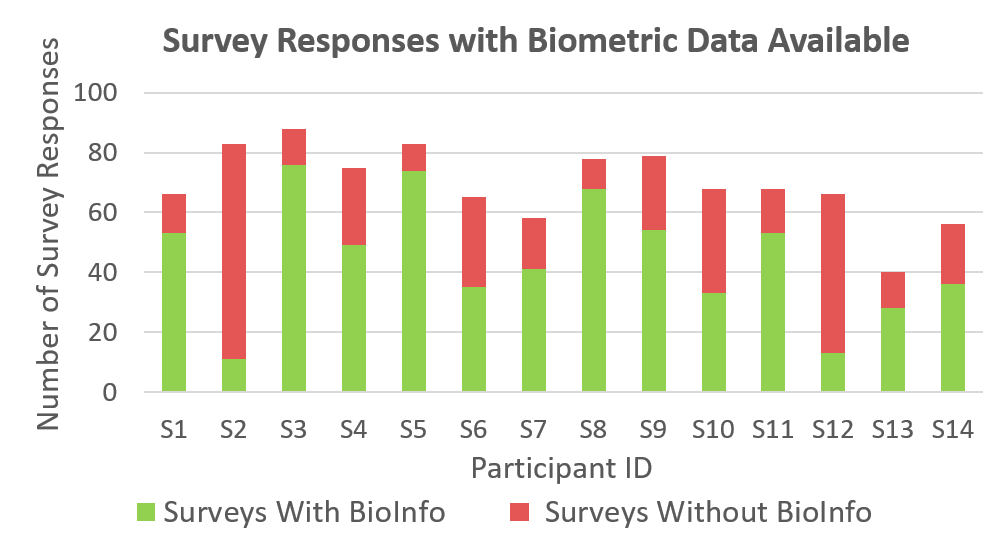
\includegraphics[width=0.8\textwidth]{DuringTheDay.png}
  \caption{The figure shows the biometric data available per each participant. Green sections represent survey responses with biometric
  data available, red sections responses with no biometric data available}
   \label{surveyBio}
   \vspace*{-4mm}
\end{figure}


\subsubsection{Feature Extraction}
We extracted features from the biometric data to provide as input to machine 
learning models. Previous 
studies~ \cite{vorburger05,zuger2015interruptibility} identify time windows as an 
important factor that impacts the prediction accuracy of a classifier. We 
considered many time windows from the literature on biometric 
analysis~\cite{zuger18}, ranging from 10 seconds to 3 hours. Specifically, we 
considered the following time windows: \textit{10sec, 20sec, 30sec, 45sec, 
1min, 2min, 3min, 5min, 7.5min, 10min, 20min, 30min, 45min, 1hour, 2hour, 
3hour}.

From the start time of each survey response, we look back the amount of time 
that corresponds to each time window and we create features for all of the 
biometric data available in that time window. For example, if a participant 
started a survey response at 11:05am, for the 30min time window, we create 
features using all of the available biometric data from 10:35am to 11:05am. 
If there is a large portion ($\geq$50\%) of data missing (either because of a recording issue or because of low quality data) from the time window considered, then the time window is marked as missing. In this case, features are imputed based on the mean of other samples of the same feature for that participant. This is an effective and commonly used technique, which is preferable to the alternative of deletion as it preserves our already small sample size~\cite{hawthorne2005imputing}.
For each time window, we calculate 10 statistical measurements from the 
biometric data to create 10 distinct features. Specifically, the 10 
statistical measurements are: mean, standard deviation, variance, median, 
25\textsuperscript{th} percentile, 75\textsuperscript{th} percentile, interquartile range, maximum, minimum, and 
range. Thus, for each survey response, we generate a large number of 
corresponding features based on three factors: biometric measurement, time 
window, and statistical measurement. In addition to these biometric 
features, we also considered the time of day in which the questions were 
asked. These features are created to predict the responses described by the 
ground truth. To attempt to account for inter-participant differences, we normalized all features on a per-participant basis.

\begin{table}
  \centering
      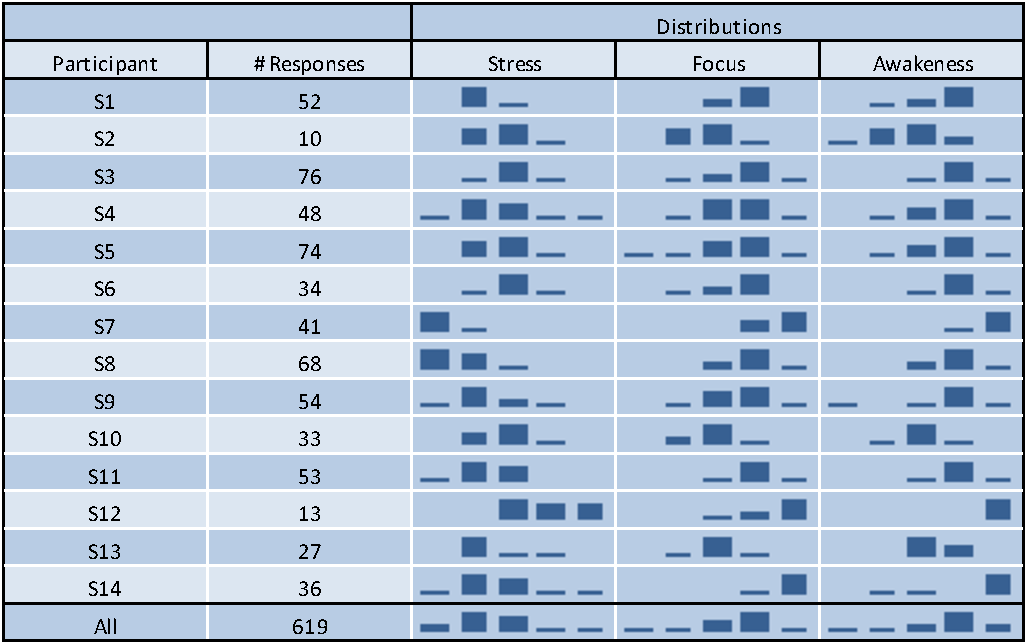
\includegraphics[width=0.8\textwidth]{distributiontable.pdf}
  \caption{The distribution of the responses of each participant to the three questions asked during the day are shown. Each bar in the histograms represent one of the \ref{five} values on the 5-point Likert scale we asked participants to respond with, where the far left side of the histograms are 1/Not at all, and the far right sides are 5/Extremely}
   \label{responseDistribution}
   %\vspace*{-2mm}
\end{table}

\subsubsection{Response Transformations}
Table~\ref{responseDistribution} illustrates the distribution of responses from each participant for each of the three survey questions (listed in Section~\ref{sec:Surveys}). The figure shows that there is a notable imbalance in the distribution of the self-reported responses provided by the participants. Most participants did not use all five points of the five-point Likert scale in their responses, and the distributions tend to skew toward one side or the other, depending on the question. Given 
this distribution and based on our earlier observation that the participants tended to adhere to a baseline reporting level for stress and awakeness, we elected to simplify the problem from \rev{five} classes to \rev{two}. This transformation enables us to more easily represent patterns in the data, such as when a participant fluctuates from a normal to high stress level. To perform this transformation, \rev{we began by calculating the median response value for each participant and each question}. We classified each response below the median as 0 (`negative') and each response above the median as 1 (`positive'). The distribution for the stress question skewed left, so we included the median values in the `positive' class (i.e. `stressed'), while the distributions for focus and awakeness skewed right, so we included those median values in the `negative' class (i.e. `not focused', `not awake').

With this method, we transformed the survey data into a two-point scale, representing  negative or positive responses for each of the three human aspects of interests (e.g., not stressed or stressed). 

\subsubsection{Oversampling}
Even after binarizing the responses as described in the previous section, we found the distribution of responses was still quite imbalanced for many of our participants. This can be seen in the distribution columns in Table \ref{tab:accuracy}. To mitigate this effect, we applied random oversampling to our training sets, which artificially rebalances the dataset by creating randomly replicated data in the minority class. This technique has commonly been used  in previous studies on unbalanced datasets \cite{chawla2004,yap2014}.

\begin{comment}
\begin{table}[h]
	\begin{centering}
	\small\addtolength{\tabcolsep}{-1pt}
    \begin{tabular}{llll}
      \hline
      Variable & K & \# Estimators & Minimum Samples Split \\
      \hline
      Stress & 300 & 100 & 4\\
      Focus & 200 & 50 & 4\\
      Awakeness & 800 & 100 & 4\\
      \hline
    \end{tabular}
    \caption{The hyperparameters selected by grid search analysis to tune our random forest models. K refers to the number of features selected.}    \label{tab:hyperparams}
    \end{centering}
\end{table}
\end{comment}


\subsection{Selecting a Classifier Algorithm}

\rev{Many different algorithms can be used to build a classifier.} To select an
algorithm, we compared multiple classifiers using the popular machine learning library scikit-learn~\cite{pedregosa11},  evaluating each one by using leave-one-out cross validation. Our analysis showed that random forest outperforms all other classifiers, including Na\"ive Bayes, decision trees, support vector machine, and a multilayer perceptron neural network. For the remainder of this paper, we refer to a random forest classifier.%\\[-0.1cm]
% for stress they were (minimum samples for split = 4, # of estimators = 100, max features = 0.5, k=300), for focus they were (minimum samples for split = 4, # of estimators = 50, max features = 0.5, k=200), and for awakeness they were (minimum samples for split = 4, # of estimators = 100, max features = 0.25, k=800)



\begin{table*}[h]
  \centering
  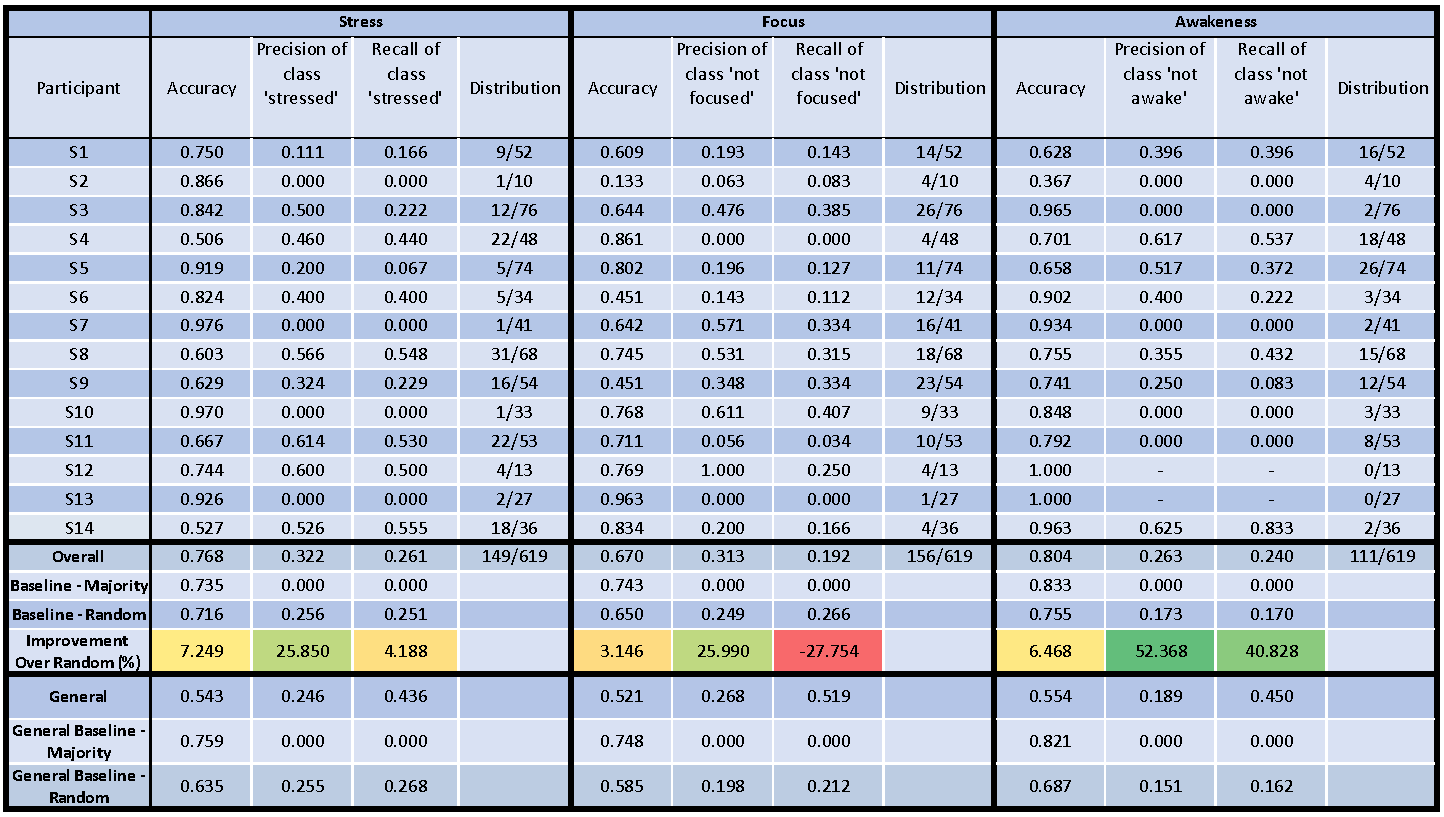
\includegraphics[width=1.0\textwidth]{rq1performance_v2.pdf}
  \caption{Results of predictions using the individual models. The distribution columns show the proportion of the minority class out of the total number of responses for each of the three variables. The baseline rows represents the averaged results of our baseline classifiers. The general row shows the averaged results of our models trained on all participants.}\label{tab:accuracy}%\todo{revise caption}}
  \vspace*{-4mm}
\end{table*}

\subsection{Individual Classifiers}
%\noindent\textit{Results of Individual Classifiers}\\
Since peoples' experience of stress, focus, and awakeness (as well as
their physiological manifestations) can vary substantially
(e.g.,~\cite{Hernandez11}), we first trained and evaluated individual classifiers
for each participant (as opposed to a general one for all
participants) using leave-one-out cross validation. The results of our analysis are reported in
Table~\ref{tab:accuracy}. For our analysis, we report values of
accuracy, one of the most commonly used metric to compare performance,
as well as precision and recall of the classes of interest:
`stressed', `not focused', and `not awake'. Since the imbalance in the
data can lead to high accuracy values if a classifier always just
predicts the most likely/frequent class while ignoring the class of
higher importance and interest, precision and recall of the class of
interest are also important to
consider~\cite{yap2014,bhattacharyya_data_2011,Hernandez11}.

\rev{Besides} our results, for the purposes of comparison\rev{,} we also present two commonly used baselines in this table - a majority classifier, which always predicts the larger of the two classes considered, and a stratified random classifier which randomly chooses between the two classes, but with a proportional bias towards the larger class.

For some users (i.e., S1. as seen in Table \ref{responseDistribution}), the imbalance in their data was so extreme that even after adjusting by oversampling\rev{, we were not able} to create a reasonable classifier. These scenarios are difficult to predict\rev{,} as any classifier will not have enough variance in its training data for the 'stressed' situation to adequately distinguish it from the non-stressed case.


% However, the imbalance in the data can lead to a classifier with high accuracy if it always just predicts the more likely class while ignoring the class of higher importance and interest in our case (i.e. stressed, not focused, not awake). Therefore, we further report the precision and recall for the three classes 'stressed', 'not focused' and 'not awake'. 


Overall, we were able to use extracted physiological features to
predict all three aspects with reasonable accuracy, precision, and
recall. We present a comparison between the averaged results of our individual classifiers and those of the baseline stratified random \rev{classifier} in the ``Improvement Over Random'' row of Table \ref{tab:accuracy}. This is calculated as the difference between the overall average and the baseline results, divided by the baseline results (for example, $\frac{Acc_{Overall} - Acc_{Random}}{Acc_{Random}}$). We do not compare our results with the majority classifier directly as this classifier achieved precision and recall scores of zero when predicting stress, lack of focus, and lack of awakeness, making a meaningful comparison \rev{unfeasible}. The improvement percentages demonstrate that the predictions made by our classifiers are much better than random after correcting for the imbalance in our dataset.

While the individually trained classifiers
improved on average across all participants upon the baseline in all
cases except in recall of `not focused', the improvement was
substantially higher for awakeness (52.4\% improvement in precision,
40.8\% in recall, and 6.5\% in accuracy) than for stress or focus. In addition,
the performance of the individually trained classifiers varied greatly
across participants. While some participants showed a large
improvement, for others the baseline performed much better than the
individually trained classifier. For instance, for predicting
`stressed', the individual classifiers improved upon the baseline for
S4, S6, S8, S11, S12, and S14 with a maximum improvement of 152.0\% in
precision and 111.1\% in recall for S12, while they did worse for S1,
S3, S5, S7, S9, S10, and S13, and in the worst cases did not correctly
predict a single instance of `stressed'. Typically, users that have the
lowest precision and recall values are those where the data is the
most imbalanced.\\[-0.1cm]
% We attribute these discrepancies to the large differences in response distributions between participants, as well as to the subjectivity of self-reporting.
%
%(improvement: 8\% precision, 1\% recall, 8\% accuracy), the individual performance varied greatly among participants. Some participants showed negligible difference in comparison to the baseline classifier, e.g. subject ..., while others showed a large improvement, e.g. subject ...
%\begin{table}[h!]
%\begin{centering}
%\begin{tabular}{lll}
%\hline
%Participant & Recall Improvement (\%) & Precision Improvement (\%)\\
%\hline
%S12 & 184.6 & 88.4 \\
%S6 & 66.7 & 85.8 \\
%S11 & 50.0 & 44.4 \\
%S8 & 32.4 & 26.7 \\
%S14 & 14.7 & 9.8 \\
%S4 & 5.6 & 5.5 \\
%S9 & -55.4 & -46.8 \\
%S3 & -90.0 & -82.1 \\
%S1 & -100.0 & -100.0 \\
%S5 & -100.0 & -100.0 \\
%S7 & -100.0 & -100.0 \\
%S10 & -100.0 & -100.0 \\
%S13 & -100.0 & -100.0\\
%S2 & - & -\\
%\hline
%\end{tabular}
%\caption{Percentage improvement in recall and precision for stress, using our approach compared to the baseline, on an individual level. For participant 2, the baseline achieved a precision and recall of 0, thus the improvement is undefined}
%\end{centering}
%\label{tab:indImprovement}
%\end{table}


\subsection{Feature Selection and Importance}
%\noindent\textit{Feature Selection and Importance}\\
There are a large variety of features that can be (and have been) calculated in previous research for each of the basic measurements listed in Table~\ref{signals}, such as the mean, standard deviation, maximum, and interquartile range. In addition, each of these metrics can be combined with the various time windows captured of a basic measurement, resulting in a large feature space. To reduce the feature space, we experimented with multiple feature selection methods, including selecting the top k highest correlated features by various metrics such as mutual information, Pearson's correlation coefficient, ANOVA's F-value, as well as wrapper methods such as recursive feature elimination, optimizing mean decrease accuracy by iteratively permuting features, and only selecting features that exceed a certain Gini importance threshold. We found that all methods produced similar results with respect to accuracy, precision, and recall for the individual models. Ultimately, we elected not to utilize any feature selection in order to simplify our approach, as we found there to be minimal differences in performance between the techniques, and the random forest algorithm is capable of (and robust for) handling datasets with many features.

%Respiration rate is also highly important for stress (#3 , 14.4%) but I'm not sure what previous works say about correlation with stress
Overall, the features that were selected as the important ones for the individual models based on the random forest algorithm varied greatly across participants. Yet, some feature categories were considered to be important more frequently than others. Table~\ref{tab:featureImportance} shows the averaged Gini importance for the feature categories used for predicting stress. Heart rate variability proved to be an important measure for all of the aspects of interest, ranking as the most important feature category for both stress and awakeness, and the second most important one for focus. This is not surprising, as heart rate variability and skin temperature have been shown in several previous studies to be possible indicators for stress levels~\cite{dishman2000stress,mcduff16,kataoka00}. We also found blood pulse wave to be an important indicator for both focus and awakeness, but less important for stress, while respiration rate was important in stress and focus but not awakeness. Besides these mentioned feature categories, there was great variation in which measures were important to which of the three aspects. This shows that there is a clear benefit to having multiple biometric streams available for predicting stress, focus and awakeness.\\[-0.1cm]


\begin{table}[h!]
  \begin{centering}
  \begin{tabular}{llll}
    \hline
    Feature Category & Stress & Focus & Awakeness\\
    \hline
    Heart Rate Variability & 18.3\% & 13\% & 13.6\%\\
    Blood Pulse Wave & 10\% & 14.2\% & 13.1\%\\
    Heart Rate & 8.7\% & 12.6\% & 10.3\%\\
    Skin Temperature & 15.7\% & 9.8\% & 10\%\\
    Galvanic Skin Response & 6.6\% & 8.2\% & 5.1\%\\
    Respiration Rate & 14.8\% & 12.7\% & 10\%\\
    Oxygen Saturation & 5.6\% & 4.3\% & 2\%\\ 
    Energy Expenditure & 6\% & 7.7\% & 4.8\%\\
    Activity & 4.6\% & 7.8\% & 7.6\%\\
    Steps & 1.7\% & 0.8\% & 0.9\%\\
    Time of Day & 0\% & 0.1\% & 0.5\%\\
    \hline
  \end{tabular}
  \caption{The averaged Gini importance of each feature category, per response variable.}
  \label{tab:featureImportance}
  \end{centering}
  \vspace*{-2mm}
\end{table}

\subsection{Individual vs.\ General Model}
%\noindent\textit{Individual vs.\ General Model}\\
Individual models are trained specifically for each individual and thus require a data collection period before they are capable of making accurate predictions. On the other hand, the idea of general models is to be able to train them on already collected data and then  to be able to apply them even to new and unseen individuals, thus overcoming the cold-start problem. Given the large individual differences in biometrics, training a general model to achieve an adequate accuracy for new individuals is not necessarily possible. 

To examine the performance of a general model for our participants, we trained three general models, one for focus, one for awakeness and one for stress. We roughly followed the same procedure as for the individual models. Due to the larger amount of data available in the general case, we used the more common random undersampling, which randomly selects elements in the majority class to exclude from the dataset, instead of random oversampling to balance the distribution of the dataset. The models were trained on the datasets of 13 of the 14 participants, and then evaluated on the dataset of the last (leave-one-participant-out cross-validation), repeating this process for all 14 participants. 

The bottom \rev{three} rows of Table \ref{tab:accuracy} present the averaged performance results for this approach in terms of accuracy, precision, and recall, as well as the results of baseline stratified random and majority classifiers following the same leave-one-group-out cross-validation procedure. Although the averaged precision and recall are comparable or better than those of the averaged individual results, this was at the cost of a large decrease in overall accuracy.  Upon closer investigation into the performance of the general model when testing on each participant, we found that individually trained models for each participant performed much better than a general model trained over all participants. Using stress as an example, for participant S12, for whom we saw the greatest increase compared to the baseline in individual models, the general model was unable to predict a single instance of `stressed' correctly. This is consistent with our expectations because biometric features are highly specific to individuals.


%\todo{put the content of the following sentence somewhere into the discussion; We attribute these discrepancies to the large differences in response distributions between participants, as well as to the subjectivity of self-reporting.}


%%%!TEX root = bioPrediction_main.tex

\subsection{Minimum Number of Training Samples}\label{secLearningCurve}
Collecting experience samples from users is expensive, since participants 
are being interrupted several times a day and have to answer the survey. 
To minimize the number of samples to be collected from participants, we 
examined how the performance of individual classifiers changes over the 
number of samples used to train the classifier.

Participants in our study had varying levels of responsiveness to the 
experience sampling ranging from 10 to 76 (see Figure~
\ref{responseDistribution}).
%Answering Reviewer 2's concern: Why only 10 participants? What was the rationale for the cut-off selected? 
To answer this research question we analyze the maximum number of responses \textbf{all} analyzed participants have to train the model. Since some participants have a very small number of maximum answers (ten being the lowest) we excluded the four participants with the least number of responses for this analysis.
%To maintain a certain generalizability while 
%also being able to examine a range of sample numbers for training the 
%classifier, we removed the four participants with the least number of 
%samples for this analysis. 
As a result, we obtained a corpus of analysis where all participants have a 
higher number of responses (34 being the lowest), which allows us to examine 
the learning curve of the classifiers for a larger number of training data points. For our 
analysis, we thus performed a leave-one-out cross validation with random 
sample sets of size 1 to 33 and calculated the average through all folds of 
the validation.

For each of the three productivity-related aspects, we are again more 
interested in predicting when a worker is stressed, not awake, or not 
focused, the less common class in all three cases. Since the less common 
class can be very small, we weighted each participants' classifier 
performance by the percentage of the samples in this smaller class.

\begin{figure}
  \centering
          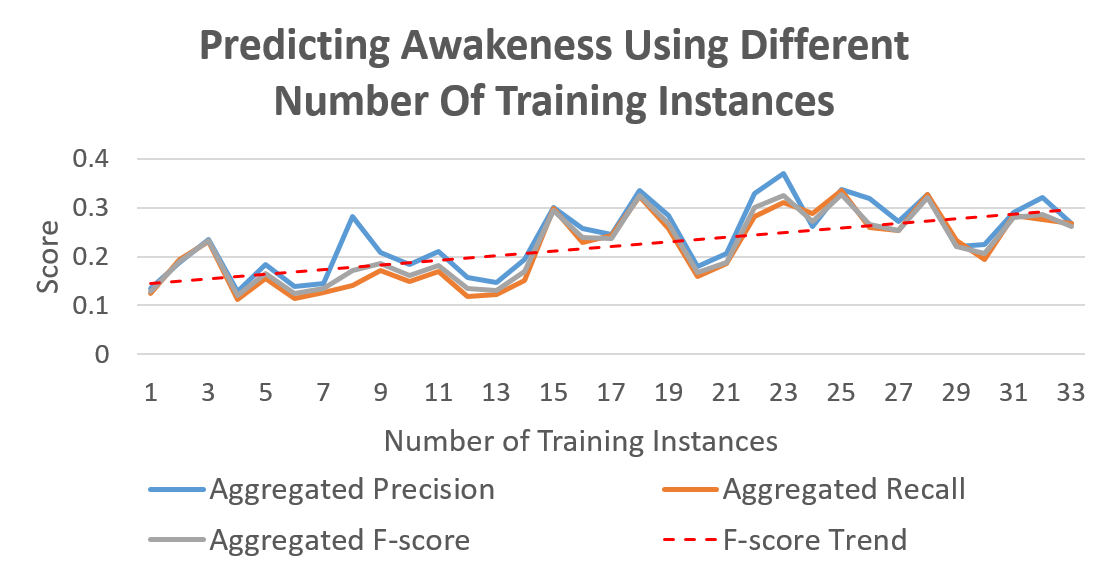
\includegraphics[width=0.5\textwidth]{20180912AwakenessLC2.png}
  \caption{Performance of the per participant trained awakeness classifiers, measured in precision, recall (sensitivity), and F-score. The dotted red line represents the F-score trend.}\label{fig:learningCurveInd}
  %\vspace*{-3mm}
\end{figure}

%\vspace{0.05in}
\noindent\textit{Individual Classifiers for Binary Prediction}\\
The averaged performance of all individually trained random forest classifiers for 'awake' with respect to the training sample size is presented in Figure~\ref{fig:learningCurveInd}. The trend indicates a positive correlation between the number of samples in the training set and the classifiers' F-score performance, with an overall improvement of  114\% (from 0.14 to 0.30) in the F-score between a training set of one sample to one with 33 samples. The trends for
the remaining indicators are 29\% for stress and no overall improvement for focus.%\\[-0.1cm]

%\noindent\textit{}
%When contrasting
%models trained and tested on the 
%biometric data of each user individually, against
%a general model trained and tested with the data of all users. 
%We can conclude
%that for up to 33 training samples analyzed in this study,
%the former has better performance when predicting the
%responses of each user than when training 
%a model with the data of several different users. 
%This is partially due to the 
%variability across users and the subjective nature
%of the responses (e.g.,where slightly awake for one person
%may be not awake for another). 

\begin{figure}
  \centering
      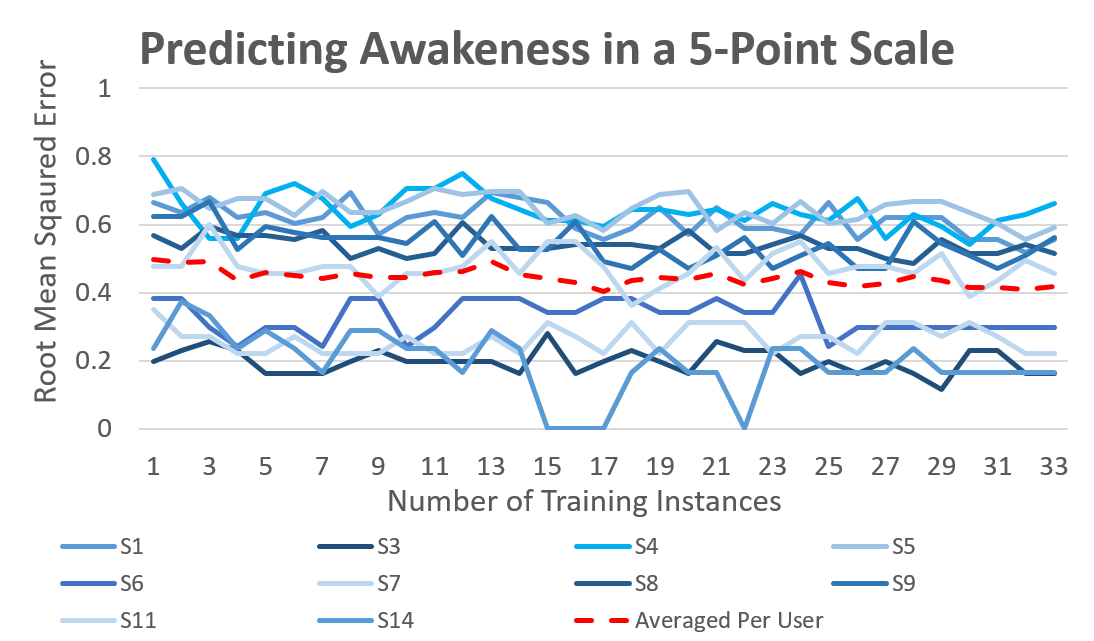
\includegraphics[width=0.5\textwidth]{20180914Awakeness5PointScaleOnly15Lines.png}
  \caption{Performance of the per participant trained classifiers for predicting 5-point awakeness, measured in root mean squared error.}
   \label{fig:learningCurve5}
\end{figure}

\noindent\textit{Predicting Five Classes}\\
In a second step, we analyzed a more fine-grained prediction using the initial 5-point Likert scale responses rather than the binarized ones as output measure. Figure~\ref{fig:learningCurve5} depicts the performance of the individually trained classifiers in terms of the root mean squared error. The root mean squared error represents the distance of the predicted from the actual value, which provides a more nuanced measure of the performance in the fine-grained prediction case. The figure shows a similar trend as for the binarized prediction, in that the root mean square error averaged over all ten participants decreases with more samples (from 0.49 to 0.41 root mean square error) and thus the performance increases. At the same time, the figure also shows that the performance results for the fine-grained prediction, again, vary substantially across participants.

\subsection{Minimum Time Window}\label{secMinimumTW}
In general, the less biometric data is needed to accurately predict a certain outcome measure, the easier and faster the analysis and data collection. To examine the optimal and minimum time window for the prediction of stress, focus, and awakeness, we used 16 different time windows from 10 seconds to 3 hours as depicted in Figure~\ref{timeWindows}. For our analysis, we then trained individual classifiers for each of the 16 time windows, using only features that had a time window smaller or equal to the time window rather than using all combinations of $\{Biometric Measures\} X \{Statistical Metrics\} X \{Time Windows\}$. We again used random forest and a leave-one-out cross validation to train individual classifiers. Since the number of features used for the training changed with each time window, we did not apply our feature selection in this case, but used all features available. Finally, due to the imbalance in the data, we again weighted each participants' classifier performance by the number of instances in the smaller class to calculate the average.

\begin{figure}
  \centering
      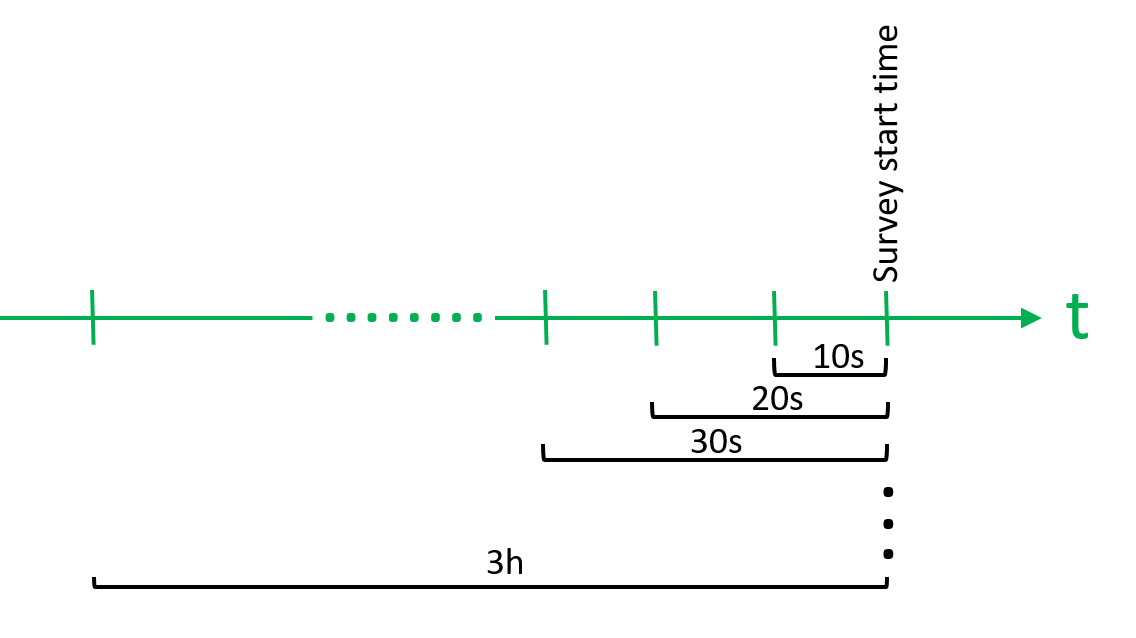
\includegraphics[width=0.4\textwidth]{timeWindows.png}
  \caption{Time windows of biometric data collected prior to each survey response: 10sec, 20sec, 30sec, 45sec, 1min, 2min, 3min, 5min, 7.5min, 10min, 20min, 30min, 45min, 1hour, 2hour, and 3hour.}
   \label{timeWindows}
\end{figure}

Figure~\ref{timeWindowsPandR} shows how the F-score changes for predicting 
`awake' over the 16 different time windows. The figure shows an increasing 
trend in the F-score, i.e. the higher the number of included time windows, 
the higher the F-score. However, there is one exception, the time window of 
1200 seconds that achieves a performance close to the one for the time 
window 10,800 seconds (3 hours), at which point all features are included. 
Overall, our results thus show that while using all time windows up to 3 
hours performs best, and outperforms the feature set that is solely based on 
a 10 second time window by 28\% (from 0.18 to 0.24), the performance for a 
time window of 1200 seconds is a good trade-off for selecting a shorter time 
window while maintaining high performance.

\begin{figure}
  \centering
      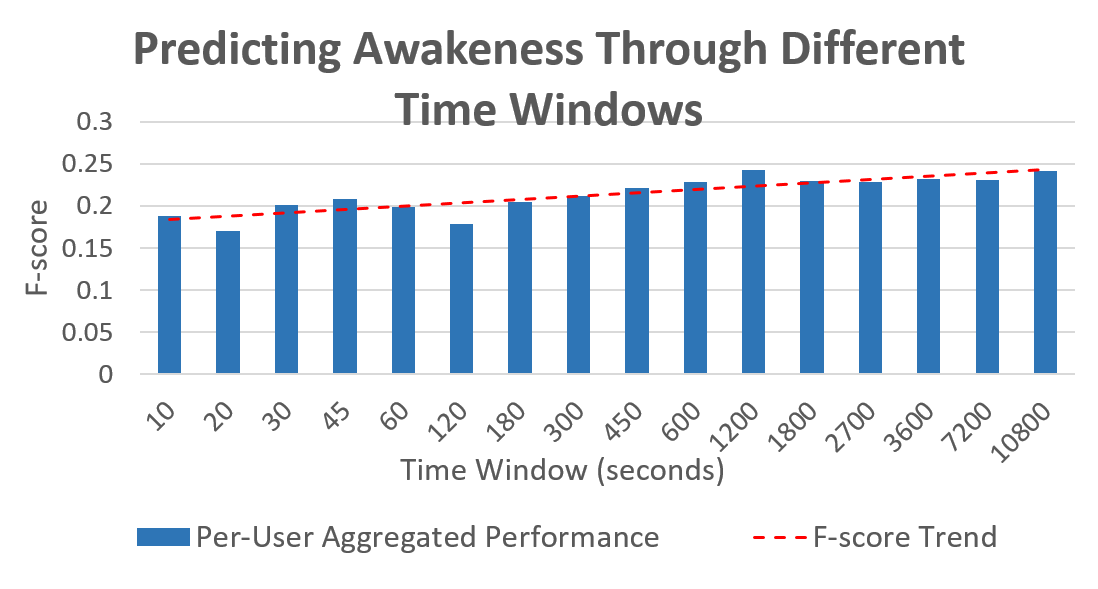
\includegraphics[width=0.5\textwidth]{20180912AwakenessTWBars.png}
  \caption{Performance (F-score) of individual classifiers trained on the different time windows to predict `awake'.}
  \label{timeWindowsPandR}
 % \vspace*{-3mm}
\end{figure}

%We also compared the performance of a model created per user against
%a model created across users.
%To calculate the performance of the model created per user,
%for each user we create a model using the features 
%related to each time window for the selected user only, 
%while in the model created with data across users,
%we trained the model with the data related to each
%particular time window of all users.
%our results show that the personalized model created
%for each user outperforms in every case
%the model created the with data across all users.

%This study
%shows that in general larger time windows predict stress,
%focus, and awakeness more precisely than 
%shorter time windows. We can also notice
%a very gentle upwards trend
%with a inflexion points at 45 seconds and 180.
%There is a peak of performance in 45 seconds, 
%time window that could be used if time is a scarce resource.
%The performance stabilizes around 180 time window
%which indicates that collecting data for a longer time
%period will not increase significantly the performance of the approach.
%The difference in performance between the 
%lowest performing and the highest performing time window is 
%less than a 10\% improvement. 


\subsection{Computer Interaction Data} \label{secCI}
Given our focus on knowledge workers (i.e., workers who generally spend a lot of time interacting with information on their computer at work), we also analyzed the use of computer interaction features to predict focus, awakeness and stress. To collect computer interaction data, we used an open source computer interaction monitor (reference omitted for double-blind.)
%the open source PersonalAnalytics project\footnote{https://github.com/sealuzh/PersonalAnalytics}  \cite{meyer18} 
to track participant's mouse and keyboard activity, as well as details about their active window. The specifics of the features tracked are listed in Table \ref{tracker}. The tracker was installed on the computers of 10 of the 14 participants, with participants S6, S10, S12, and S13 opting out of this part of the study due to privacy concerns.  Therefore, we limited this analysis to the 10 participants for whom we could calculate all features. 

\begin{table}
\begin{center}
\small\addtolength{\tabcolsep}{-1pt}
\begin{tabular}{l l}
\hline

Feature collected by tool & Description \\ 
\hline
Total keystrokes per min& Sum of all types of keystrokes \\ 
Normal keystrokes per min&F[h] Not backspace and navigation \\ 
Backspace keystrokes per min& Backspace keystrokes \\ 
Navigation keystrokes per min& Arrow key keystrokes \\ 
Total clicks per min& Sum of all click types \\ 
Other clicks per min& Not right and left clicks \\ 
Left clicks per min& Left clicks \\ 
Right clicks per min& Right clicks \\ 
Scrolled distance per min& Scrolled distance in pixels \\ 
Moved distance per min& Mouse movements in pixels \\ 
Activity switches per min& Browser window title changes \\ 
Category switches per min& Activity performed category \\ 
\hline
\end{tabular}
\caption{Features collected per user by the computer interaction tracker}%~\cite{meyer18}}
\label{tracker}
\end{center}
%\vspace*{-1mm}
\end{table}

For calculating computer interaction features, we again used the aforementioned 16 time windows and scaled the computer interaction values if the time windows did not align. For our comparative analysis of the different sensing techniques---biometrics vs computer interaction---we then created two new feature sets for each participant in addition to the biometric one: one with only computer interaction features, and one with computer interaction features plus biometric features. 

Table~\ref{ciPerformance} lists the results of our analysis. The results show that in all cases, the computer interaction based model was able to improve upon the biometric model in terms of precision and recall.
%MS is removing the accuracy results because it is not what we care about and it is just making the results harder to understand
%, but not in accuracy. 
Further, we found that the combined model was the most effective model in terms of precision and recall for predicting stress and awakeness overall, but performed slightly worse than the model using only computer interaction features for focus. 
%Since we consider precision and recall for predicting the class of higher interest, i.e. stressed, not focused, not awake, to be the most important statistics when interpreting our results, we compared the models against each other by averaging these two statistics.


\begin{table}
\begin{center}
%\small\addtolength{\tabcolsep}{-1pt}
\begin{tabular}{llllll}
\hline
Model/Feature Set & Precision & Recall & F-Score \\ %& Accuracy\\
\hline
\textbf{Awakeness}\\
\hspace{3mm}Biometrics only  & 0.269 & 0.314 & 0.289 \\ %& 0.808\\
\hspace{3mm}C.I. only  & 0.425 & 0.362 & 0.391 \\ % & 0.758\\
\hspace{3mm}Biometrics + C.I. & 0.390 & 0.404 & 0.400 \\ % & 0.791 \\
\hline
\textbf{Stress}\\
\hspace{3mm}Biometrics only  & 0.270 &	0.260 & 0.265 \\ % & 0.775\\
\hspace{3mm}C.I. only & 0.290 & 0.272 & 0.281 \\ % & 0.698 \\
\hspace{3mm}Biometrics + C.I. & 0.317 & 0.286 & 0.301 \\ % & 0.712\\
\hline
\textbf{Focus}\\
\hspace{3mm}Biometrics only & 0.251 & 0.256 & 0.253 \\ % & 0.716\\
\hspace{3mm}C.I. only & 0.332 & 0.342 & 0.337 \\ % & 0.742\\
\hspace{3mm}Biometrics + C.I. & 0.340 & 0.316 & 0.328 \\ % & 0.745\\
\hline
\end{tabular}
\caption{Comparison of the performance of predicting stress, focus and awakeness using the 3 different feature sets for the 10 participants. The performance is calculated as the average of the performance of the individual classifiers. Computer Interactions is abbreviated as C.I. here for readability. Precision and recall refer to the prediction of the more important classes, i.e. `stressed', `not awake', `not focused'.}
\label{ciPerformance}
\end{center}
%\vspace*{-1mm}
\end{table}

As with the biometric models, the individual performance of both the computer interaction only models and the combined models varied quite a bit between participants. Using stress as an example again, in the computer interaction models 5 of the 10 participants saw improvements compared to the baseline, with a maximum improvement of 128\% in precision, and 78\% in recall. In the combined model for stress, 5 of the 10 participants saw improvements compared to the baseline, with a maximum improvement of 117\% in precision and 95\% in recall. Neither model was capable of correctly predicting any instances of 'stressed' for participant S7.

Since the number of features changes  depending on which feature set is used, we adjusted the feature selection parameter for each of the computer interaction and combined computer interaction/biometric models. The values reported in this section were achieved using the optimal feature selection parameters we found, which are shown in Table \ref{ciFeatureSelection}.

\begin{table}
\begin{center}
\begin{tabular}{lc}
\hline
Model/Feature Set & Number of Features Selected\\
\hline
\textbf{Stress}\\
\hspace{3mm}C.I. & 400\\
\hspace{3mm}Biometrics + C.I. & 800\\
\hline
\textbf{Focus}\\
\hspace{3mm}C.I. & 20\\
\hspace{3mm}Biometrics + C.I. & 300\\
\hline
\textbf{Awakeness}\\
\hspace{3mm}C.I. & All\\
\hspace{3mm}Biometrics + C.I. & 50\\
\hline
\end{tabular}
\caption{The optimal number of features we found to select for each of the model/feature set combinations. Computer interactions is abbreviated as C.I.}
\label{ciFeatureSelection}
\end{center}
\vspace*{-4mm}
\end{table}



%\section{Analysis and Results}

%% To evaluate the efficacy of continuously predicting a knowledge worker's stress, focus, and awakeness in the workplace, we trained and tested machine learning classifiers using a leave-one-out cross validation. For prediction, we used the features extracted from the collected data as the input data, and binarized the participants' self-reported responses on stress, focus, and awakeness into two classes each (e.g., 'stressed' and 'not stressed') to use as output measures.

\section{Observed Trends Over Time in Stress and Awakeness Levels}
\label{stressTrends}

To gain insights into how knowledge workers experience stress and awakeness over an
extended period of work, we examined the end of day survey responses
collected from each participant to see if any identifiable trends
emerged. As we noted in the last section, we did not ask
participants about focus in the end of  day surveys as focus is an 
aspect relevant at a particular moment in time rather than an aspect
for an extended period of work. We used data from 13 of the 14 participants - we excluded one participant
from this analysis as they experienced atypical stress
levels in the latter half of the study due to factors outside of our
control.

\subsection{Stress Levels}
Overall, we identified three prominent characteristics in the stress levels.
%\rev{We describe characteristics noted in the reporting of the knowledge workers about the stress they experienced over the duration of the study.}

\begin{figure}[h!]
  \centering
      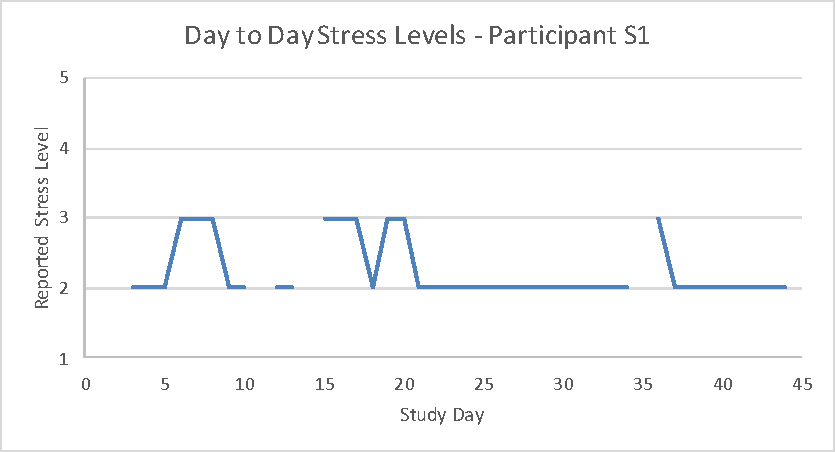
\includegraphics[width=0.7\textwidth]{s1_stress.pdf}
      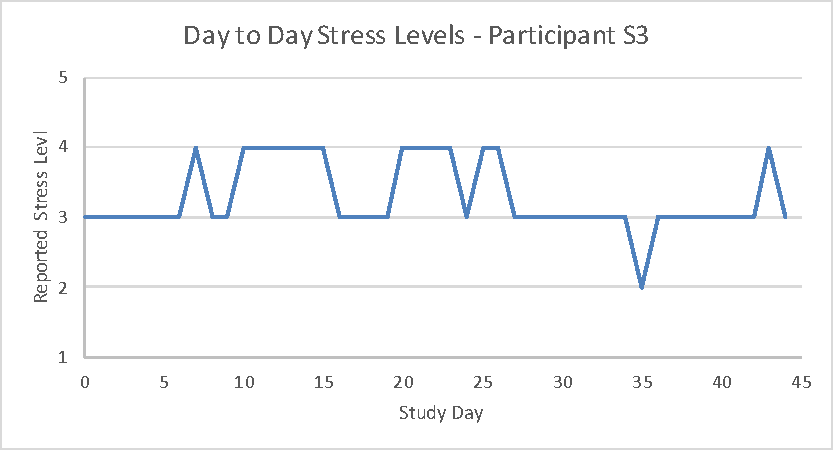
\includegraphics[width=0.7\textwidth]{s3_stress.pdf}
  \caption{The day-to-day stress levels reported by two participants (S1 and S3) are shown. The y-axis represents values on the 5-point Likert scale we asked participants to respond with ranging from 1/Not at all stressed to 5/Extremely stressed. The x-axis represents the day of the study on which the value was recorded (from 0-45). Some gaps are present in the chart for S1 as they did not report their stress level on those days.}
   \vspace*{-2mm}
   \label{fig:dailyStress}
\end{figure}


\subsubsection{Baseline Stress Levels}
%\noindent\textit{\textbf{Baseline Stress Levels.}}
Common amongst all participants was a trend to select one stress rating
far more frequently than any other. We will refer to this value as the
participant's baseline stress level. All but one participant reported
their perceived stress level for the day as their baseline stress
level more than 50\% of the time. In total, the baseline values made
up 65\% of the reported values collected from
participants. Interestingly, while participants sometimes saw periods
of sustained increases in stress, lasting as many as 6 consecutive
workdays in the most extreme case, participants would always return to
their baseline stress level at some point.


The baseline stress level varied significantly between participants. \rev{Seven}
participants (54\%) reported feeling average stress levels most frequently
(rating 3 on our scale), while \rev{five} (38\%) reported feeling little stress
(rating 2) and \rev{one} (8\%) reported feeling no stress at all (rating 1). Figure \ref{fig:dailyStress} illustrates these points using  data from two participants, showing the tendency to report and return to baseline stress levels, as well
as a distinct difference in baseline stress level (rating 2 for S1 vs rating 3 for S3). Gaps in the chart for S1 represent days for which the participant did not report their stress level.


\subsubsection{Stressful Days Tend to Cluster}
Accounting for the variance between participants perceived stress
baselines, we consider a stressful day to be one that represents a
deviation of \rev{one} or more stress levels above the participant's
baseline. Of the 93 stressful days we observed in total, we found that
39 (41\%) of these days occurred in groupings of two or more
consecutive stressful workdays. The most common size of these groups
was two workdays, while the largest group we observed was six
workdays.  The day after a stressful day is much more likely to be a
stressful day as compared to any other day with a 0.55 average increase
over baseline, compared to 0.02 average increase over baseline.

\subsubsection{Extreme Changes in Stress Levels are Rare}
After accounting for each participant's perceived stress baseline, we
examined the frequency of deviations from the baseline. We found that
participants were far more likely to report a stress level that was
within \rev{one} point of their baseline, than to report a stress level 2 or
more points away. These extreme deviations represented only 15\% of
all reported values, which differed from the \rev{participant's} baseline. As
well, the majority (78\%) of these deviations came from just two
participants. This suggests that some people may be less resilient to
the stress of the workplace than others. For most participants,
extremely stressful days were few and far between.

\subsection{Awakeness}
We applied the same analyses described above to the \rev{self-reported} awakeness levels of our participants. Compared with the reported stress levels, we observed the same trend of participants reporting one baseline far more commonly than any other. We did not find there to be a significant correlation between reported stress and awakeness levels. Overall, \rev{participant's} awakeness levels fluctuated significantly less than their stress levels (73.1\% of reports were at the baseline level, compared to 65.1\% for stress, p < 0.05). Participants were unlikely to experience days with heightened (above baseline) awakeness. Such days made up only 6.0\% of the total observed \rev{workdays} across all participant. Most of these days came from one participant, S2, who reported 15 heightened awakeness days compared to the next highest, S13 with four. Large deviations (>1 point deviation) from each participants baseline awakeness levels were extremely uncommon, accounting for only \rev{nine} (2.1\%) of our total observations. Similarly to what we observed with high stress days, low awakeness days frequently came in clusters of two or three days in a row. Given that the immediately preceding day was a low awakeness day\rev{;} a given day was 228.2\% more likely to be a low awakeness day than when considering any day at random (p < 0.0001).


\begin{table}[]
    \centering
\rev{\begin{tabularx}{\textwidth}{|c|c c c|c c c|}
    \hline
        &
        \multicolumn{3}{c|}{Stress} & 
        \multicolumn{3}{c|}{Awakeness} \\
        \hline
        \textbf{Variable} & \centering
        \textbf{\rev{F.E.E.}}& \textbf{p-value} & \textbf{\rev{C.I. (95\%)}} & \centering \textbf{\rev{F.E.E.}}  & \textbf{p-value} & \textbf{\rev{C.I. (95\%)}}\\
        \hline
        Monday & \centering -0.033 & 0.745 & \rev{$(-0.234, 0.167)$} & \centering -0.058 & 0.497 & \rev{$(-0.227, 0.110)$}\\
        Tuesday & \centering 0.028 & 0.773 & \rev{$(-0.164, 0.221)$} & \centering 0.036 & 0.662 & \rev{$(-0.126, 0.198)$}\\
        Wednesday & \centering 0.163 & 0.100 & \rev{$(-0.031, 0.357)$} & \centering -0.018 & 0.830 & \rev{$(-0.181, 0.145)$}\\
        Thursday & \centering 0.022 & 0.821 & \rev{$(-0.169, 0.213)$} & \centering 0.076 & 0.927 & \rev{$(-0.085, 0.238)$}\\
        Friday & \centering 0.082 & 0.473 & \rev{$(-0.142, 0.306)$} & \centering -0.178 & 0.025 & \rev{$(-0.334, -0.022)$}\\
        Month End & \centering 0.044 & 0.687 & \rev{$(-0.171, 0.259)$} & \centering -0.082 & 0.374 & \rev{$(-0.263, 0.099)$}\\
        \hline
    \end{tabularx}
    \caption{\rev{Fixed effects estimates (F.E.E.), 95\% confidence intervals and associated p-values for the explanatory variables (day of week and proximity to month end) that we examined in our linear mixed model analysis.}}    \label{tab:mixedModel}}
\end{table}





\subsection{Explaining Fluctuations}
In an attempt to explain some of the fluctuations in stress and awakeness that our participants were experiencing, we created a linear mixed model with the self-reported daily stress and awakeness levels as dependent variables and the participants as random effects. We experimented with day of the week and proximity to beginning or end of month as possible explanatory variables. Ultimately, the analysis showed that none of the variables that we examined had a significant explanatory power with respect to our participants perceived stress levels.
For awakeness, we found  that there was a small (\rev{fixed effects estimate}: -0.178) yet significant decrease in awakeness levels on Fridays in particular. Table \ref{tab:mixedModel} shows some of the detailed results of these analyses. These results show the difficulty of explaining a person's stress and awakeness via simple measures, and point to the need for additional instrumentation and data collection if we are to successfully understand and make predictions about these human aspects in the workplace.




\section{Predicting Stress, Focus and Awakeness in the Moment}
% random forest best
\label{secOverallAccuracy}

To investigate whether stress, focus and awakeness can be predicted in
the moment based on biometric measures,
we investigated classifiers trained
for each individual and across all participants. We report on the effectiveness of
these classifiers and the features that are important in predicting stress, focus
and awakeness.

\subsection{Data Preparation}

\rev{In a machine learning context, data preparation and utilization is an essential part of the proposed solution. To prepare} the collected data for use in training and testing \rev{our proposed} machine learning models, we performed \rev{the following} steps.


\subsubsection{Data Cleaning}
All data recorded by the Everion is associated with a quality score ranging from 0-1 that is calculated using proprietary methods. In accordance with the recommendations of Biovotion,
to prevent our results from being effected by erroneous data we set a quality threshold of 0.5 and discarded any data gathered which had a quality rating below this threshold. 

\subsubsection{Data Linking}

We linked the collected biometric data and survey responses for each participant. Linking the data is necessary to construct training and test datasets for use in creating and evaluating machine learning models.

To link the data, we look back one hour from the start time of each survey response for
available biometric data.  For example, if a participant started a survey response at 11:05am, we look for biometric data from between 10:05am to 11:05am. If no biometric data was recorded in the hour time window, we exclude the survey response from the dataset. Otherwise, we consider the survey response to have associated biometric data.

There are several reasons for a survey response to lack associated biometric data:
\begin{itemize}
\item The participant was not wearing the Everion in the hour before beginning the survey.
\item The Everion was not recording data in the hour before the participant began the survey (e.g., due to low battery).
\item Biometric data was not being uploaded successfully to the server.
%\item Compatibility issues between the sensor and the OS tracking the participant's data
%\item Issues accessing the data uploaded by the participants
\end{itemize}

Figure~\ref{surveyBio} illustrates the number of survey responses with associated biometric data for each study participant. 
%This was added to address REviewer 2's concern: Is it correct that the maximum number of responses should have been 112 on the surveys?
The total number of responses per participant is affected by their response rate and by the number days out-of-office (e.g., vacations, holidays, etc.). 
Participant S2 and S12 have particularly low numbers of usable survey responses. In each of these cases, the issue related to biometric data not being uploaded successfully to the server.

\begin{figure}
  \centering
      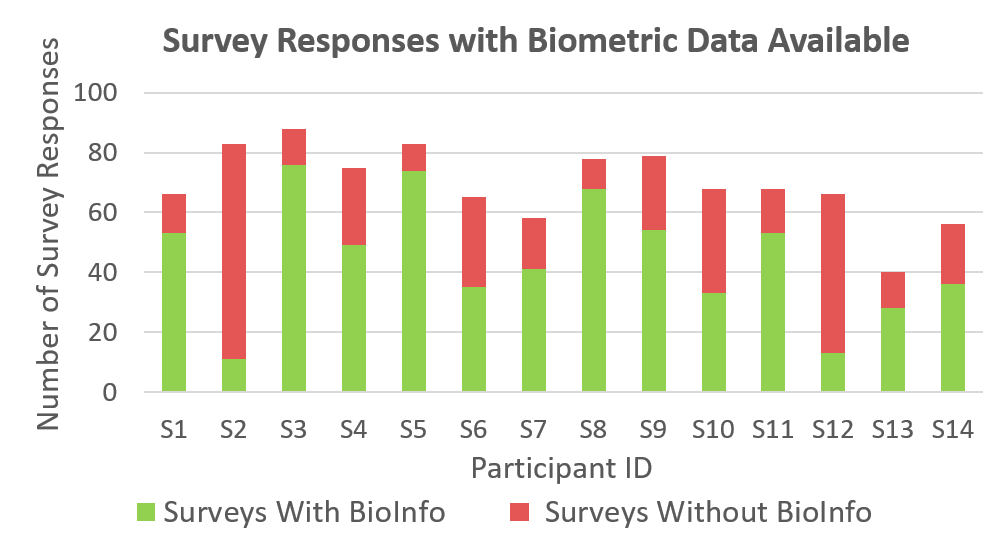
\includegraphics[width=0.8\textwidth]{DuringTheDay.png}
  \caption{The figure shows the biometric data available per each participant. Green sections represent survey responses with biometric
  data available, red sections responses with no biometric data available}
   \label{surveyBio}
   \vspace*{-4mm}
\end{figure}


\subsubsection{Feature Extraction}
We extracted features from the biometric data to provide as input to machine 
learning models. Previous 
studies~ \cite{vorburger05,zuger2015interruptibility} identify time windows as an 
important factor that impacts the prediction accuracy of a classifier. We 
considered many time windows from the literature on biometric 
analysis~\cite{zuger18}, ranging from 10 seconds to 3 hours. Specifically, we 
considered the following time windows: \textit{10sec, 20sec, 30sec, 45sec, 
1min, 2min, 3min, 5min, 7.5min, 10min, 20min, 30min, 45min, 1hour, 2hour, 
3hour}.

From the start time of each survey response, we look back the amount of time 
that corresponds to each time window and we create features for all of the 
biometric data available in that time window. For example, if a participant 
started a survey response at 11:05am, for the 30min time window, we create 
features using all of the available biometric data from 10:35am to 11:05am. 
If there is a large portion ($\geq$50\%) of data missing (either because of a recording issue or because of low quality data) from the time window considered, then the time window is marked as missing. In this case, features are imputed based on the mean of other samples of the same feature for that participant. This is an effective and commonly used technique, which is preferable to the alternative of deletion as it preserves our already small sample size~\cite{hawthorne2005imputing}.
For each time window, we calculate 10 statistical measurements from the 
biometric data to create 10 distinct features. Specifically, the 10 
statistical measurements are: mean, standard deviation, variance, median, 
25\textsuperscript{th} percentile, 75\textsuperscript{th} percentile, interquartile range, maximum, minimum, and 
range. Thus, for each survey response, we generate a large number of 
corresponding features based on three factors: biometric measurement, time 
window, and statistical measurement. In addition to these biometric 
features, we also considered the time of day in which the questions were 
asked. These features are created to predict the responses described by the 
ground truth. To attempt to account for inter-participant differences, we normalized all features on a per-participant basis.

\begin{table}
  \centering
      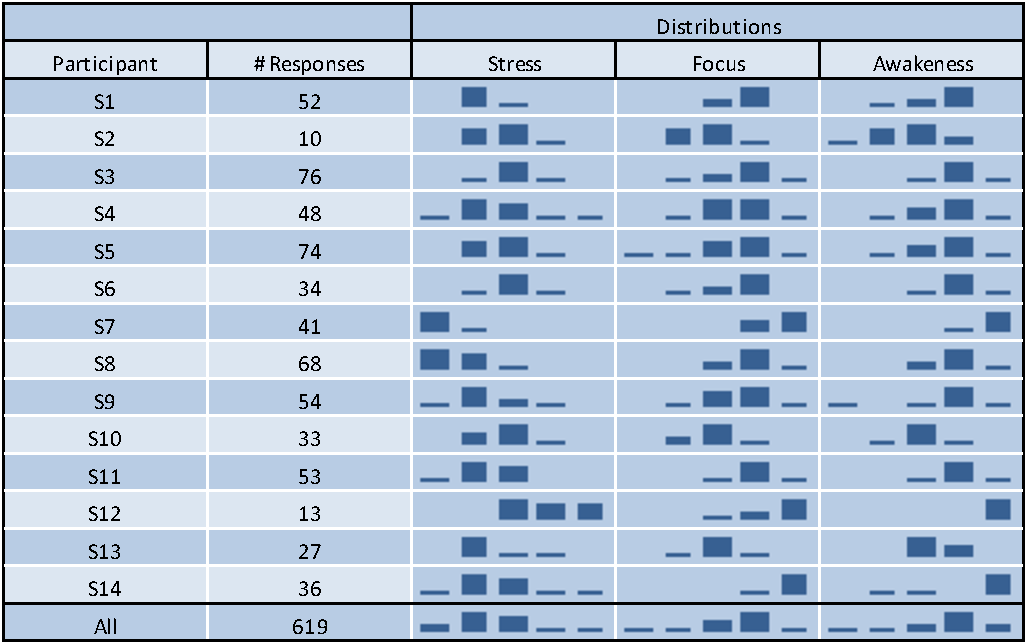
\includegraphics[width=0.8\textwidth]{distributiontable.pdf}
  \caption{The distribution of the responses of each participant to the three questions asked during the day are shown. Each bar in the histograms represent one of the \ref{five} values on the 5-point Likert scale we asked participants to respond with, where the far left side of the histograms are 1/Not at all, and the far right sides are 5/Extremely}
   \label{responseDistribution}
   %\vspace*{-2mm}
\end{table}

\subsubsection{Response Transformations}
Table~\ref{responseDistribution} illustrates the distribution of responses from each participant for each of the three survey questions (listed in Section~\ref{sec:Surveys}). The figure shows that there is a notable imbalance in the distribution of the self-reported responses provided by the participants. Most participants did not use all five points of the five-point Likert scale in their responses, and the distributions tend to skew toward one side or the other, depending on the question. Given 
this distribution and based on our earlier observation that the participants tended to adhere to a baseline reporting level for stress and awakeness, we elected to simplify the problem from \rev{five} classes to \rev{two}. This transformation enables us to more easily represent patterns in the data, such as when a participant fluctuates from a normal to high stress level. To perform this transformation, \rev{we began by calculating the median response value for each participant and each question}. We classified each response below the median as 0 (`negative') and each response above the median as 1 (`positive'). The distribution for the stress question skewed left, so we included the median values in the `positive' class (i.e. `stressed'), while the distributions for focus and awakeness skewed right, so we included those median values in the `negative' class (i.e. `not focused', `not awake').

With this method, we transformed the survey data into a two-point scale, representing  negative or positive responses for each of the three human aspects of interests (e.g., not stressed or stressed). 

\subsubsection{Oversampling}
Even after binarizing the responses as described in the previous section, we found the distribution of responses was still quite imbalanced for many of our participants. This can be seen in the distribution columns in Table \ref{tab:accuracy}. To mitigate this effect, we applied random oversampling to our training sets, which artificially rebalances the dataset by creating randomly replicated data in the minority class. This technique has commonly been used  in previous studies on unbalanced datasets \cite{chawla2004,yap2014}.

\begin{comment}
\begin{table}[h]
	\begin{centering}
	\small\addtolength{\tabcolsep}{-1pt}
    \begin{tabular}{llll}
      \hline
      Variable & K & \# Estimators & Minimum Samples Split \\
      \hline
      Stress & 300 & 100 & 4\\
      Focus & 200 & 50 & 4\\
      Awakeness & 800 & 100 & 4\\
      \hline
    \end{tabular}
    \caption{The hyperparameters selected by grid search analysis to tune our random forest models. K refers to the number of features selected.}    \label{tab:hyperparams}
    \end{centering}
\end{table}
\end{comment}


\subsection{Selecting a Classifier Algorithm}

\rev{Many different algorithms can be used to build a classifier.} To select an
algorithm, we compared multiple classifiers using the popular machine learning library scikit-learn~\cite{pedregosa11},  evaluating each one by using leave-one-out cross validation. Our analysis showed that random forest outperforms all other classifiers, including Na\"ive Bayes, decision trees, support vector machine, and a multilayer perceptron neural network. For the remainder of this paper, we refer to a random forest classifier.%\\[-0.1cm]
% for stress they were (minimum samples for split = 4, # of estimators = 100, max features = 0.5, k=300), for focus they were (minimum samples for split = 4, # of estimators = 50, max features = 0.5, k=200), and for awakeness they were (minimum samples for split = 4, # of estimators = 100, max features = 0.25, k=800)



\begin{table*}[h]
  \centering
  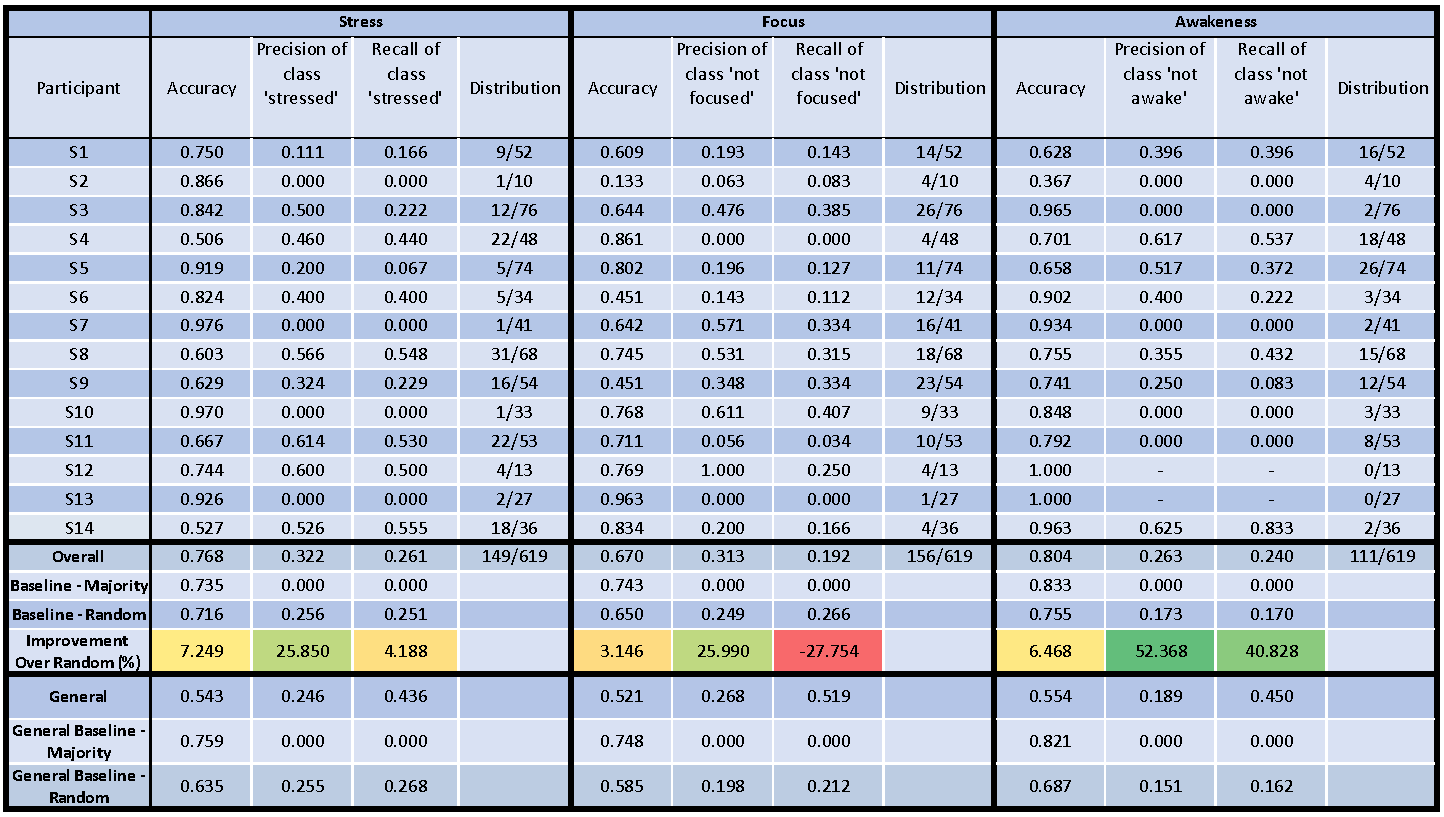
\includegraphics[width=1.0\textwidth]{rq1performance_v2.pdf}
  \caption{Results of predictions using the individual models. The distribution columns show the proportion of the minority class out of the total number of responses for each of the three variables. The baseline rows represents the averaged results of our baseline classifiers. The general row shows the averaged results of our models trained on all participants.}\label{tab:accuracy}%\todo{revise caption}}
  \vspace*{-4mm}
\end{table*}

\subsection{Individual Classifiers}
%\noindent\textit{Results of Individual Classifiers}\\
Since peoples' experience of stress, focus, and awakeness (as well as
their physiological manifestations) can vary substantially
(e.g.,~\cite{Hernandez11}), we first trained and evaluated individual classifiers
for each participant (as opposed to a general one for all
participants) using leave-one-out cross validation. The results of our analysis are reported in
Table~\ref{tab:accuracy}. For our analysis, we report values of
accuracy, one of the most commonly used metric to compare performance,
as well as precision and recall of the classes of interest:
`stressed', `not focused', and `not awake'. Since the imbalance in the
data can lead to high accuracy values if a classifier always just
predicts the most likely/frequent class while ignoring the class of
higher importance and interest, precision and recall of the class of
interest are also important to
consider~\cite{yap2014,bhattacharyya_data_2011,Hernandez11}.

\rev{Besides} our results, for the purposes of comparison\rev{,} we also present two commonly used baselines in this table - a majority classifier, which always predicts the larger of the two classes considered, and a stratified random classifier which randomly chooses between the two classes, but with a proportional bias towards the larger class.

For some users (i.e., S1. as seen in Table \ref{responseDistribution}), the imbalance in their data was so extreme that even after adjusting by oversampling\rev{, we were not able} to create a reasonable classifier. These scenarios are difficult to predict\rev{,} as any classifier will not have enough variance in its training data for the 'stressed' situation to adequately distinguish it from the non-stressed case.


% However, the imbalance in the data can lead to a classifier with high accuracy if it always just predicts the more likely class while ignoring the class of higher importance and interest in our case (i.e. stressed, not focused, not awake). Therefore, we further report the precision and recall for the three classes 'stressed', 'not focused' and 'not awake'. 


Overall, we were able to use extracted physiological features to
predict all three aspects with reasonable accuracy, precision, and
recall. We present a comparison between the averaged results of our individual classifiers and those of the baseline stratified random \rev{classifier} in the ``Improvement Over Random'' row of Table \ref{tab:accuracy}. This is calculated as the difference between the overall average and the baseline results, divided by the baseline results (for example, $\frac{Acc_{Overall} - Acc_{Random}}{Acc_{Random}}$). We do not compare our results with the majority classifier directly as this classifier achieved precision and recall scores of zero when predicting stress, lack of focus, and lack of awakeness, making a meaningful comparison \rev{unfeasible}. The improvement percentages demonstrate that the predictions made by our classifiers are much better than random after correcting for the imbalance in our dataset.

While the individually trained classifiers
improved on average across all participants upon the baseline in all
cases except in recall of `not focused', the improvement was
substantially higher for awakeness (52.4\% improvement in precision,
40.8\% in recall, and 6.5\% in accuracy) than for stress or focus. In addition,
the performance of the individually trained classifiers varied greatly
across participants. While some participants showed a large
improvement, for others the baseline performed much better than the
individually trained classifier. For instance, for predicting
`stressed', the individual classifiers improved upon the baseline for
S4, S6, S8, S11, S12, and S14 with a maximum improvement of 152.0\% in
precision and 111.1\% in recall for S12, while they did worse for S1,
S3, S5, S7, S9, S10, and S13, and in the worst cases did not correctly
predict a single instance of `stressed'. Typically, users that have the
lowest precision and recall values are those where the data is the
most imbalanced.\\[-0.1cm]
% We attribute these discrepancies to the large differences in response distributions between participants, as well as to the subjectivity of self-reporting.
%
%(improvement: 8\% precision, 1\% recall, 8\% accuracy), the individual performance varied greatly among participants. Some participants showed negligible difference in comparison to the baseline classifier, e.g. subject ..., while others showed a large improvement, e.g. subject ...
%\begin{table}[h!]
%\begin{centering}
%\begin{tabular}{lll}
%\hline
%Participant & Recall Improvement (\%) & Precision Improvement (\%)\\
%\hline
%S12 & 184.6 & 88.4 \\
%S6 & 66.7 & 85.8 \\
%S11 & 50.0 & 44.4 \\
%S8 & 32.4 & 26.7 \\
%S14 & 14.7 & 9.8 \\
%S4 & 5.6 & 5.5 \\
%S9 & -55.4 & -46.8 \\
%S3 & -90.0 & -82.1 \\
%S1 & -100.0 & -100.0 \\
%S5 & -100.0 & -100.0 \\
%S7 & -100.0 & -100.0 \\
%S10 & -100.0 & -100.0 \\
%S13 & -100.0 & -100.0\\
%S2 & - & -\\
%\hline
%\end{tabular}
%\caption{Percentage improvement in recall and precision for stress, using our approach compared to the baseline, on an individual level. For participant 2, the baseline achieved a precision and recall of 0, thus the improvement is undefined}
%\end{centering}
%\label{tab:indImprovement}
%\end{table}


\subsection{Feature Selection and Importance}
%\noindent\textit{Feature Selection and Importance}\\
There are a large variety of features that can be (and have been) calculated in previous research for each of the basic measurements listed in Table~\ref{signals}, such as the mean, standard deviation, maximum, and interquartile range. In addition, each of these metrics can be combined with the various time windows captured of a basic measurement, resulting in a large feature space. To reduce the feature space, we experimented with multiple feature selection methods, including selecting the top k highest correlated features by various metrics such as mutual information, Pearson's correlation coefficient, ANOVA's F-value, as well as wrapper methods such as recursive feature elimination, optimizing mean decrease accuracy by iteratively permuting features, and only selecting features that exceed a certain Gini importance threshold. We found that all methods produced similar results with respect to accuracy, precision, and recall for the individual models. Ultimately, we elected not to utilize any feature selection in order to simplify our approach, as we found there to be minimal differences in performance between the techniques, and the random forest algorithm is capable of (and robust for) handling datasets with many features.

%Respiration rate is also highly important for stress (#3 , 14.4%) but I'm not sure what previous works say about correlation with stress
Overall, the features that were selected as the important ones for the individual models based on the random forest algorithm varied greatly across participants. Yet, some feature categories were considered to be important more frequently than others. Table~\ref{tab:featureImportance} shows the averaged Gini importance for the feature categories used for predicting stress. Heart rate variability proved to be an important measure for all of the aspects of interest, ranking as the most important feature category for both stress and awakeness, and the second most important one for focus. This is not surprising, as heart rate variability and skin temperature have been shown in several previous studies to be possible indicators for stress levels~\cite{dishman2000stress,mcduff16,kataoka00}. We also found blood pulse wave to be an important indicator for both focus and awakeness, but less important for stress, while respiration rate was important in stress and focus but not awakeness. Besides these mentioned feature categories, there was great variation in which measures were important to which of the three aspects. This shows that there is a clear benefit to having multiple biometric streams available for predicting stress, focus and awakeness.\\[-0.1cm]


\begin{table}[h!]
  \begin{centering}
  \begin{tabular}{llll}
    \hline
    Feature Category & Stress & Focus & Awakeness\\
    \hline
    Heart Rate Variability & 18.3\% & 13\% & 13.6\%\\
    Blood Pulse Wave & 10\% & 14.2\% & 13.1\%\\
    Heart Rate & 8.7\% & 12.6\% & 10.3\%\\
    Skin Temperature & 15.7\% & 9.8\% & 10\%\\
    Galvanic Skin Response & 6.6\% & 8.2\% & 5.1\%\\
    Respiration Rate & 14.8\% & 12.7\% & 10\%\\
    Oxygen Saturation & 5.6\% & 4.3\% & 2\%\\ 
    Energy Expenditure & 6\% & 7.7\% & 4.8\%\\
    Activity & 4.6\% & 7.8\% & 7.6\%\\
    Steps & 1.7\% & 0.8\% & 0.9\%\\
    Time of Day & 0\% & 0.1\% & 0.5\%\\
    \hline
  \end{tabular}
  \caption{The averaged Gini importance of each feature category, per response variable.}
  \label{tab:featureImportance}
  \end{centering}
  \vspace*{-2mm}
\end{table}

\subsection{Individual vs.\ General Model}
%\noindent\textit{Individual vs.\ General Model}\\
Individual models are trained specifically for each individual and thus require a data collection period before they are capable of making accurate predictions. On the other hand, the idea of general models is to be able to train them on already collected data and then  to be able to apply them even to new and unseen individuals, thus overcoming the cold-start problem. Given the large individual differences in biometrics, training a general model to achieve an adequate accuracy for new individuals is not necessarily possible. 

To examine the performance of a general model for our participants, we trained three general models, one for focus, one for awakeness and one for stress. We roughly followed the same procedure as for the individual models. Due to the larger amount of data available in the general case, we used the more common random undersampling, which randomly selects elements in the majority class to exclude from the dataset, instead of random oversampling to balance the distribution of the dataset. The models were trained on the datasets of 13 of the 14 participants, and then evaluated on the dataset of the last (leave-one-participant-out cross-validation), repeating this process for all 14 participants. 

The bottom \rev{three} rows of Table \ref{tab:accuracy} present the averaged performance results for this approach in terms of accuracy, precision, and recall, as well as the results of baseline stratified random and majority classifiers following the same leave-one-group-out cross-validation procedure. Although the averaged precision and recall are comparable or better than those of the averaged individual results, this was at the cost of a large decrease in overall accuracy.  Upon closer investigation into the performance of the general model when testing on each participant, we found that individually trained models for each participant performed much better than a general model trained over all participants. Using stress as an example, for participant S12, for whom we saw the greatest increase compared to the baseline in individual models, the general model was unable to predict a single instance of `stressed' correctly. This is consistent with our expectations because biometric features are highly specific to individuals.


%\todo{put the content of the following sentence somewhere into the discussion; We attribute these discrepancies to the large differences in response distributions between participants, as well as to the subjectivity of self-reporting.}


%%%!TEX root = bioPrediction_main.tex

\subsection{Minimum Number of Training Samples}\label{secLearningCurve}
Collecting experience samples from users is expensive, since participants 
are being interrupted several times a day and have to answer the survey. 
To minimize the number of samples to be collected from participants, we 
examined how the performance of individual classifiers changes over the 
number of samples used to train the classifier.

Participants in our study had varying levels of responsiveness to the 
experience sampling ranging from 10 to 76 (see Figure~
\ref{responseDistribution}).
%Answering Reviewer 2's concern: Why only 10 participants? What was the rationale for the cut-off selected? 
To answer this research question we analyze the maximum number of responses \textbf{all} analyzed participants have to train the model. Since some participants have a very small number of maximum answers (ten being the lowest) we excluded the four participants with the least number of responses for this analysis.
%To maintain a certain generalizability while 
%also being able to examine a range of sample numbers for training the 
%classifier, we removed the four participants with the least number of 
%samples for this analysis. 
As a result, we obtained a corpus of analysis where all participants have a 
higher number of responses (34 being the lowest), which allows us to examine 
the learning curve of the classifiers for a larger number of training data points. For our 
analysis, we thus performed a leave-one-out cross validation with random 
sample sets of size 1 to 33 and calculated the average through all folds of 
the validation.

For each of the three productivity-related aspects, we are again more 
interested in predicting when a worker is stressed, not awake, or not 
focused, the less common class in all three cases. Since the less common 
class can be very small, we weighted each participants' classifier 
performance by the percentage of the samples in this smaller class.

\begin{figure}
  \centering
          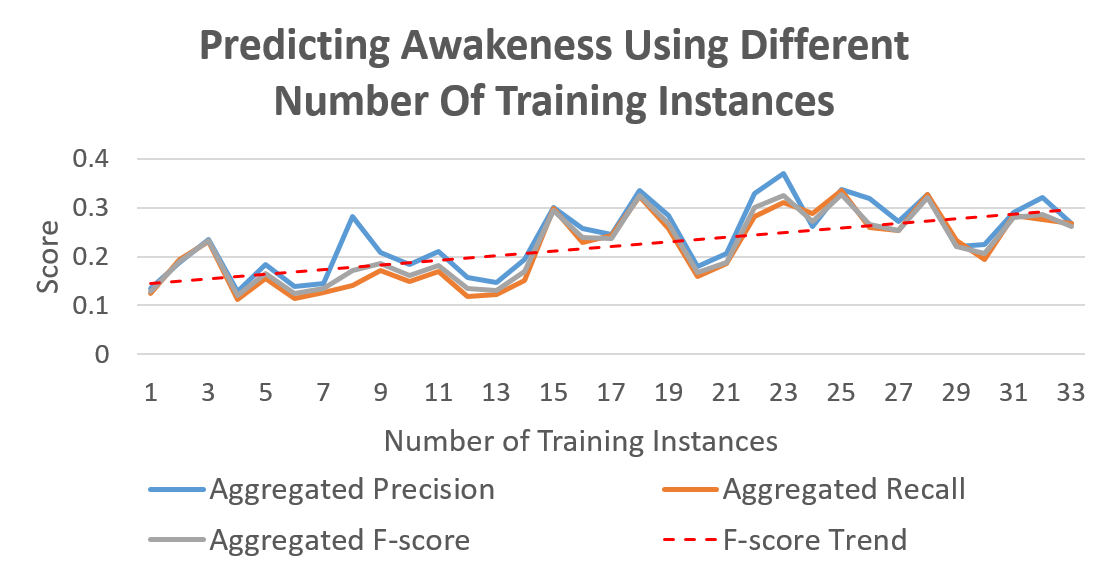
\includegraphics[width=0.5\textwidth]{20180912AwakenessLC2.png}
  \caption{Performance of the per participant trained awakeness classifiers, measured in precision, recall (sensitivity), and F-score. The dotted red line represents the F-score trend.}\label{fig:learningCurveInd}
  %\vspace*{-3mm}
\end{figure}

%\vspace{0.05in}
\noindent\textit{Individual Classifiers for Binary Prediction}\\
The averaged performance of all individually trained random forest classifiers for 'awake' with respect to the training sample size is presented in Figure~\ref{fig:learningCurveInd}. The trend indicates a positive correlation between the number of samples in the training set and the classifiers' F-score performance, with an overall improvement of  114\% (from 0.14 to 0.30) in the F-score between a training set of one sample to one with 33 samples. The trends for
the remaining indicators are 29\% for stress and no overall improvement for focus.%\\[-0.1cm]

%\noindent\textit{}
%When contrasting
%models trained and tested on the 
%biometric data of each user individually, against
%a general model trained and tested with the data of all users. 
%We can conclude
%that for up to 33 training samples analyzed in this study,
%the former has better performance when predicting the
%responses of each user than when training 
%a model with the data of several different users. 
%This is partially due to the 
%variability across users and the subjective nature
%of the responses (e.g.,where slightly awake for one person
%may be not awake for another). 

\begin{figure}
  \centering
      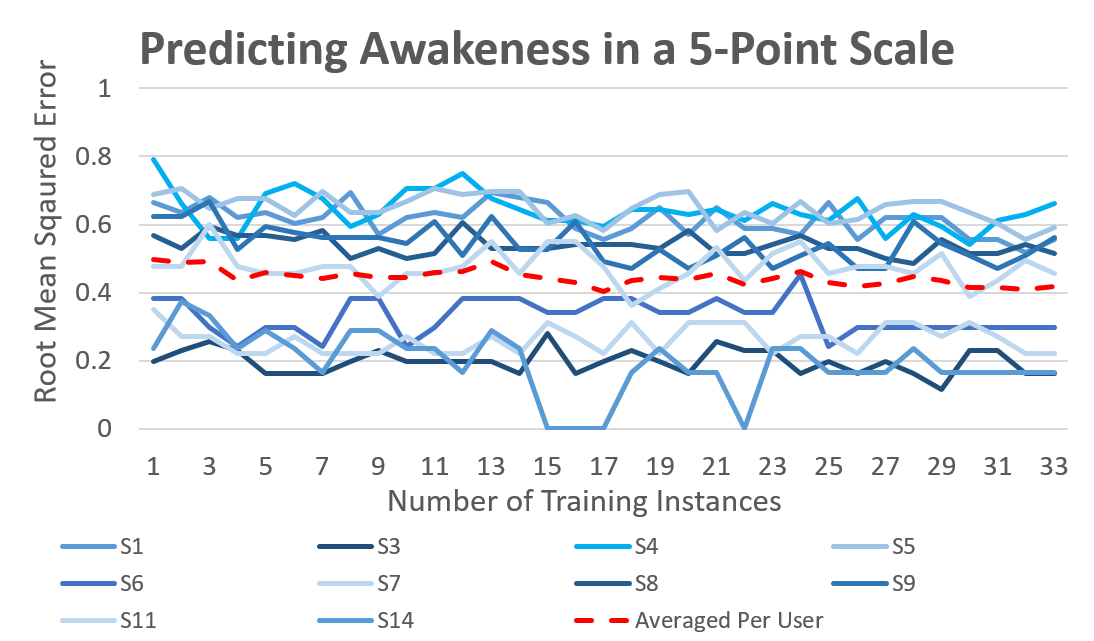
\includegraphics[width=0.5\textwidth]{20180914Awakeness5PointScaleOnly15Lines.png}
  \caption{Performance of the per participant trained classifiers for predicting 5-point awakeness, measured in root mean squared error.}
   \label{fig:learningCurve5}
\end{figure}

\noindent\textit{Predicting Five Classes}\\
In a second step, we analyzed a more fine-grained prediction using the initial 5-point Likert scale responses rather than the binarized ones as output measure. Figure~\ref{fig:learningCurve5} depicts the performance of the individually trained classifiers in terms of the root mean squared error. The root mean squared error represents the distance of the predicted from the actual value, which provides a more nuanced measure of the performance in the fine-grained prediction case. The figure shows a similar trend as for the binarized prediction, in that the root mean square error averaged over all ten participants decreases with more samples (from 0.49 to 0.41 root mean square error) and thus the performance increases. At the same time, the figure also shows that the performance results for the fine-grained prediction, again, vary substantially across participants.

\subsection{Minimum Time Window}\label{secMinimumTW}
In general, the less biometric data is needed to accurately predict a certain outcome measure, the easier and faster the analysis and data collection. To examine the optimal and minimum time window for the prediction of stress, focus, and awakeness, we used 16 different time windows from 10 seconds to 3 hours as depicted in Figure~\ref{timeWindows}. For our analysis, we then trained individual classifiers for each of the 16 time windows, using only features that had a time window smaller or equal to the time window rather than using all combinations of $\{Biometric Measures\} X \{Statistical Metrics\} X \{Time Windows\}$. We again used random forest and a leave-one-out cross validation to train individual classifiers. Since the number of features used for the training changed with each time window, we did not apply our feature selection in this case, but used all features available. Finally, due to the imbalance in the data, we again weighted each participants' classifier performance by the number of instances in the smaller class to calculate the average.

\begin{figure}
  \centering
      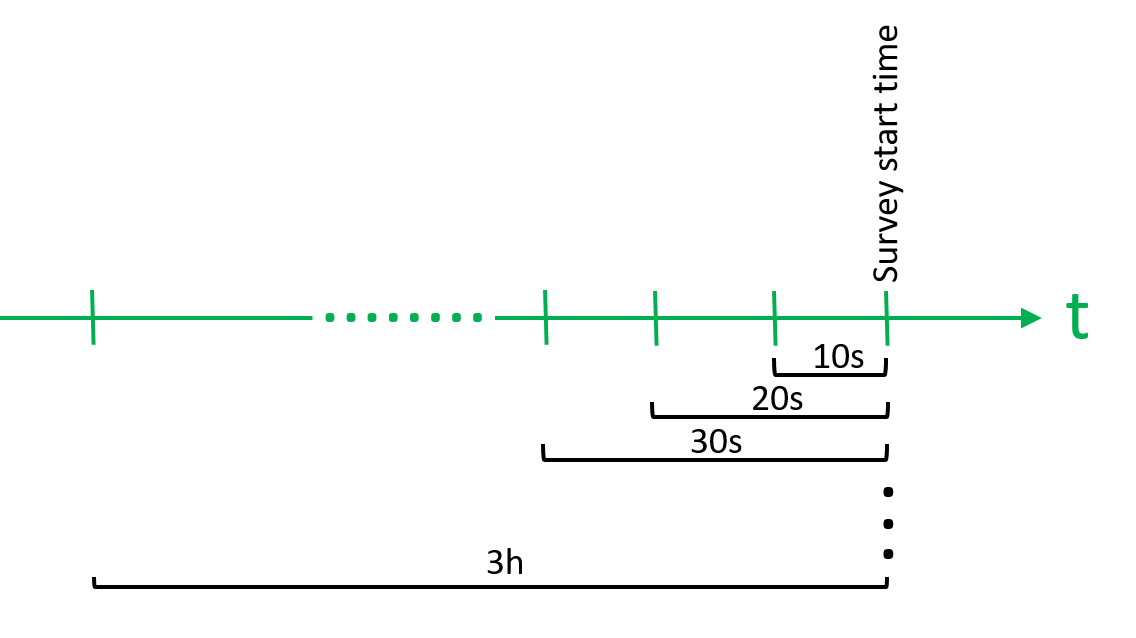
\includegraphics[width=0.4\textwidth]{timeWindows.png}
  \caption{Time windows of biometric data collected prior to each survey response: 10sec, 20sec, 30sec, 45sec, 1min, 2min, 3min, 5min, 7.5min, 10min, 20min, 30min, 45min, 1hour, 2hour, and 3hour.}
   \label{timeWindows}
\end{figure}

Figure~\ref{timeWindowsPandR} shows how the F-score changes for predicting 
`awake' over the 16 different time windows. The figure shows an increasing 
trend in the F-score, i.e. the higher the number of included time windows, 
the higher the F-score. However, there is one exception, the time window of 
1200 seconds that achieves a performance close to the one for the time 
window 10,800 seconds (3 hours), at which point all features are included. 
Overall, our results thus show that while using all time windows up to 3 
hours performs best, and outperforms the feature set that is solely based on 
a 10 second time window by 28\% (from 0.18 to 0.24), the performance for a 
time window of 1200 seconds is a good trade-off for selecting a shorter time 
window while maintaining high performance.

\begin{figure}
  \centering
      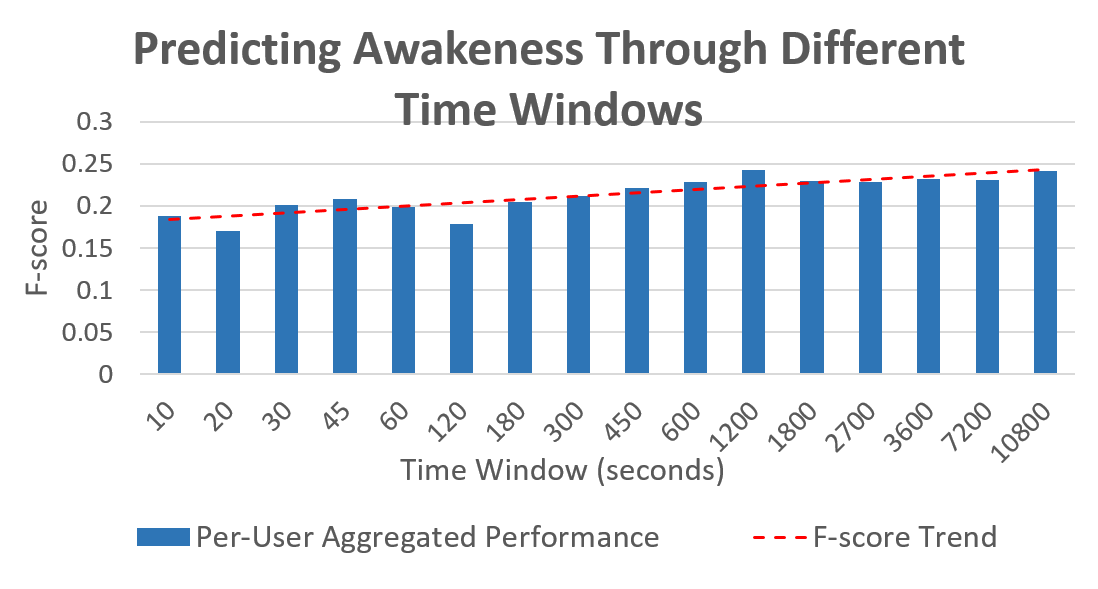
\includegraphics[width=0.5\textwidth]{20180912AwakenessTWBars.png}
  \caption{Performance (F-score) of individual classifiers trained on the different time windows to predict `awake'.}
  \label{timeWindowsPandR}
 % \vspace*{-3mm}
\end{figure}

%We also compared the performance of a model created per user against
%a model created across users.
%To calculate the performance of the model created per user,
%for each user we create a model using the features 
%related to each time window for the selected user only, 
%while in the model created with data across users,
%we trained the model with the data related to each
%particular time window of all users.
%our results show that the personalized model created
%for each user outperforms in every case
%the model created the with data across all users.

%This study
%shows that in general larger time windows predict stress,
%focus, and awakeness more precisely than 
%shorter time windows. We can also notice
%a very gentle upwards trend
%with a inflexion points at 45 seconds and 180.
%There is a peak of performance in 45 seconds, 
%time window that could be used if time is a scarce resource.
%The performance stabilizes around 180 time window
%which indicates that collecting data for a longer time
%period will not increase significantly the performance of the approach.
%The difference in performance between the 
%lowest performing and the highest performing time window is 
%less than a 10\% improvement. 


\subsection{Computer Interaction Data} \label{secCI}
Given our focus on knowledge workers (i.e., workers who generally spend a lot of time interacting with information on their computer at work), we also analyzed the use of computer interaction features to predict focus, awakeness and stress. To collect computer interaction data, we used an open source computer interaction monitor (reference omitted for double-blind.)
%the open source PersonalAnalytics project\footnote{https://github.com/sealuzh/PersonalAnalytics}  \cite{meyer18} 
to track participant's mouse and keyboard activity, as well as details about their active window. The specifics of the features tracked are listed in Table \ref{tracker}. The tracker was installed on the computers of 10 of the 14 participants, with participants S6, S10, S12, and S13 opting out of this part of the study due to privacy concerns.  Therefore, we limited this analysis to the 10 participants for whom we could calculate all features. 

\begin{table}
\begin{center}
\small\addtolength{\tabcolsep}{-1pt}
\begin{tabular}{l l}
\hline

Feature collected by tool & Description \\ 
\hline
Total keystrokes per min& Sum of all types of keystrokes \\ 
Normal keystrokes per min&F[h] Not backspace and navigation \\ 
Backspace keystrokes per min& Backspace keystrokes \\ 
Navigation keystrokes per min& Arrow key keystrokes \\ 
Total clicks per min& Sum of all click types \\ 
Other clicks per min& Not right and left clicks \\ 
Left clicks per min& Left clicks \\ 
Right clicks per min& Right clicks \\ 
Scrolled distance per min& Scrolled distance in pixels \\ 
Moved distance per min& Mouse movements in pixels \\ 
Activity switches per min& Browser window title changes \\ 
Category switches per min& Activity performed category \\ 
\hline
\end{tabular}
\caption{Features collected per user by the computer interaction tracker}%~\cite{meyer18}}
\label{tracker}
\end{center}
%\vspace*{-1mm}
\end{table}

For calculating computer interaction features, we again used the aforementioned 16 time windows and scaled the computer interaction values if the time windows did not align. For our comparative analysis of the different sensing techniques---biometrics vs computer interaction---we then created two new feature sets for each participant in addition to the biometric one: one with only computer interaction features, and one with computer interaction features plus biometric features. 

Table~\ref{ciPerformance} lists the results of our analysis. The results show that in all cases, the computer interaction based model was able to improve upon the biometric model in terms of precision and recall.
%MS is removing the accuracy results because it is not what we care about and it is just making the results harder to understand
%, but not in accuracy. 
Further, we found that the combined model was the most effective model in terms of precision and recall for predicting stress and awakeness overall, but performed slightly worse than the model using only computer interaction features for focus. 
%Since we consider precision and recall for predicting the class of higher interest, i.e. stressed, not focused, not awake, to be the most important statistics when interpreting our results, we compared the models against each other by averaging these two statistics.


\begin{table}
\begin{center}
%\small\addtolength{\tabcolsep}{-1pt}
\begin{tabular}{llllll}
\hline
Model/Feature Set & Precision & Recall & F-Score \\ %& Accuracy\\
\hline
\textbf{Awakeness}\\
\hspace{3mm}Biometrics only  & 0.269 & 0.314 & 0.289 \\ %& 0.808\\
\hspace{3mm}C.I. only  & 0.425 & 0.362 & 0.391 \\ % & 0.758\\
\hspace{3mm}Biometrics + C.I. & 0.390 & 0.404 & 0.400 \\ % & 0.791 \\
\hline
\textbf{Stress}\\
\hspace{3mm}Biometrics only  & 0.270 &	0.260 & 0.265 \\ % & 0.775\\
\hspace{3mm}C.I. only & 0.290 & 0.272 & 0.281 \\ % & 0.698 \\
\hspace{3mm}Biometrics + C.I. & 0.317 & 0.286 & 0.301 \\ % & 0.712\\
\hline
\textbf{Focus}\\
\hspace{3mm}Biometrics only & 0.251 & 0.256 & 0.253 \\ % & 0.716\\
\hspace{3mm}C.I. only & 0.332 & 0.342 & 0.337 \\ % & 0.742\\
\hspace{3mm}Biometrics + C.I. & 0.340 & 0.316 & 0.328 \\ % & 0.745\\
\hline
\end{tabular}
\caption{Comparison of the performance of predicting stress, focus and awakeness using the 3 different feature sets for the 10 participants. The performance is calculated as the average of the performance of the individual classifiers. Computer Interactions is abbreviated as C.I. here for readability. Precision and recall refer to the prediction of the more important classes, i.e. `stressed', `not awake', `not focused'.}
\label{ciPerformance}
\end{center}
%\vspace*{-1mm}
\end{table}

As with the biometric models, the individual performance of both the computer interaction only models and the combined models varied quite a bit between participants. Using stress as an example again, in the computer interaction models 5 of the 10 participants saw improvements compared to the baseline, with a maximum improvement of 128\% in precision, and 78\% in recall. In the combined model for stress, 5 of the 10 participants saw improvements compared to the baseline, with a maximum improvement of 117\% in precision and 95\% in recall. Neither model was capable of correctly predicting any instances of 'stressed' for participant S7.

Since the number of features changes  depending on which feature set is used, we adjusted the feature selection parameter for each of the computer interaction and combined computer interaction/biometric models. The values reported in this section were achieved using the optimal feature selection parameters we found, which are shown in Table \ref{ciFeatureSelection}.

\begin{table}
\begin{center}
\begin{tabular}{lc}
\hline
Model/Feature Set & Number of Features Selected\\
\hline
\textbf{Stress}\\
\hspace{3mm}C.I. & 400\\
\hspace{3mm}Biometrics + C.I. & 800\\
\hline
\textbf{Focus}\\
\hspace{3mm}C.I. & 20\\
\hspace{3mm}Biometrics + C.I. & 300\\
\hline
\textbf{Awakeness}\\
\hspace{3mm}C.I. & All\\
\hspace{3mm}Biometrics + C.I. & 50\\
\hline
\end{tabular}
\caption{The optimal number of features we found to select for each of the model/feature set combinations. Computer interactions is abbreviated as C.I.}
\label{ciFeatureSelection}
\end{center}
\vspace*{-4mm}
\end{table}



%\section{Analysis and Results}

%% To evaluate the efficacy of continuously predicting a knowledge worker's stress, focus, and awakeness in the workplace, we trained and tested machine learning classifiers using a leave-one-out cross validation. For prediction, we used the features extracted from the collected data as the input data, and binarized the participants' self-reported responses on stress, focus, and awakeness into two classes each (e.g., 'stressed' and 'not stressed') to use as output measures.

\section{Observed Trends Over Time in Stress and Awakeness Levels}
\label{stressTrends}

To gain insights into how knowledge workers experience stress and awakeness over an
extended period of work, we examined the end of day survey responses
collected from each participant to see if any identifiable trends
emerged. As we noted in the last section, we did not ask
participants about focus in the end of  day surveys as focus is an 
aspect relevant at a particular moment in time rather than an aspect
for an extended period of work. We used data from 13 of the 14 participants - we excluded one participant
from this analysis as they experienced atypical stress
levels in the latter half of the study due to factors outside of our
control.

\subsection{Stress Levels}
Overall, we identified three prominent characteristics in the stress levels.
%\rev{We describe characteristics noted in the reporting of the knowledge workers about the stress they experienced over the duration of the study.}

\begin{figure}[h!]
  \centering
      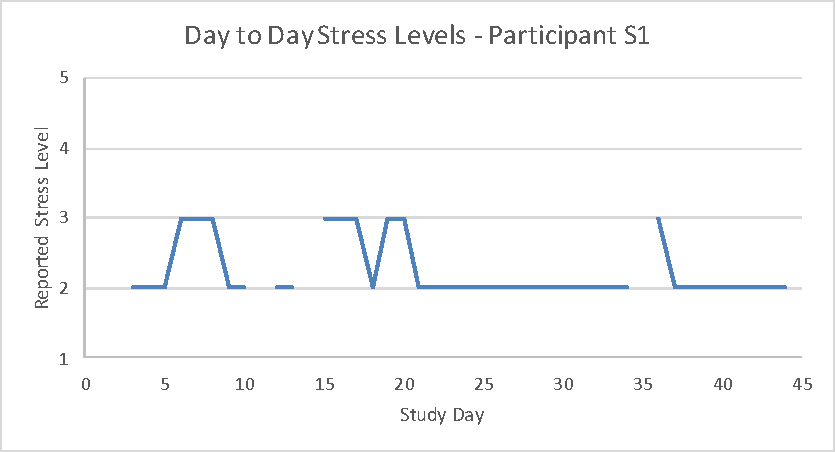
\includegraphics[width=0.7\textwidth]{s1_stress.pdf}
      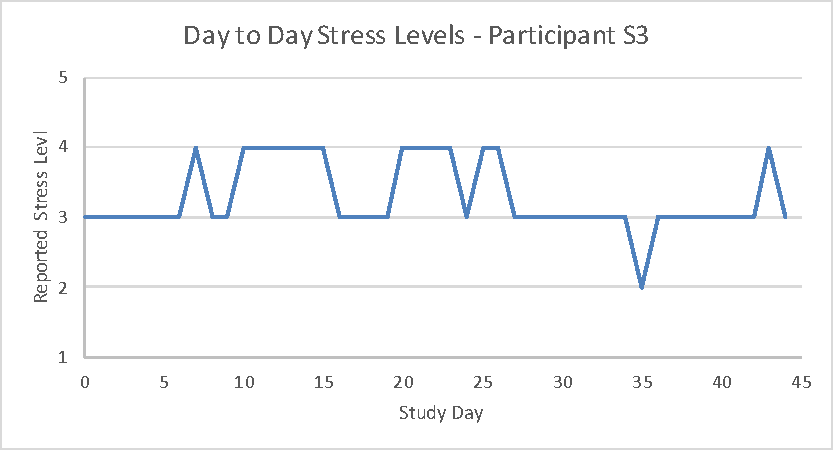
\includegraphics[width=0.7\textwidth]{s3_stress.pdf}
  \caption{The day-to-day stress levels reported by two participants (S1 and S3) are shown. The y-axis represents values on the 5-point Likert scale we asked participants to respond with ranging from 1/Not at all stressed to 5/Extremely stressed. The x-axis represents the day of the study on which the value was recorded (from 0-45). Some gaps are present in the chart for S1 as they did not report their stress level on those days.}
   \vspace*{-2mm}
   \label{fig:dailyStress}
\end{figure}


\subsubsection{Baseline Stress Levels}
%\noindent\textit{\textbf{Baseline Stress Levels.}}
Common amongst all participants was a trend to select one stress rating
far more frequently than any other. We will refer to this value as the
participant's baseline stress level. All but one participant reported
their perceived stress level for the day as their baseline stress
level more than 50\% of the time. In total, the baseline values made
up 65\% of the reported values collected from
participants. Interestingly, while participants sometimes saw periods
of sustained increases in stress, lasting as many as 6 consecutive
workdays in the most extreme case, participants would always return to
their baseline stress level at some point.


The baseline stress level varied significantly between participants. \rev{Seven}
participants (54\%) reported feeling average stress levels most frequently
(rating 3 on our scale), while \rev{five} (38\%) reported feeling little stress
(rating 2) and \rev{one} (8\%) reported feeling no stress at all (rating 1). Figure \ref{fig:dailyStress} illustrates these points using  data from two participants, showing the tendency to report and return to baseline stress levels, as well
as a distinct difference in baseline stress level (rating 2 for S1 vs rating 3 for S3). Gaps in the chart for S1 represent days for which the participant did not report their stress level.


\subsubsection{Stressful Days Tend to Cluster}
Accounting for the variance between participants perceived stress
baselines, we consider a stressful day to be one that represents a
deviation of \rev{one} or more stress levels above the participant's
baseline. Of the 93 stressful days we observed in total, we found that
39 (41\%) of these days occurred in groupings of two or more
consecutive stressful workdays. The most common size of these groups
was two workdays, while the largest group we observed was six
workdays.  The day after a stressful day is much more likely to be a
stressful day as compared to any other day with a 0.55 average increase
over baseline, compared to 0.02 average increase over baseline.

\subsubsection{Extreme Changes in Stress Levels are Rare}
After accounting for each participant's perceived stress baseline, we
examined the frequency of deviations from the baseline. We found that
participants were far more likely to report a stress level that was
within \rev{one} point of their baseline, than to report a stress level 2 or
more points away. These extreme deviations represented only 15\% of
all reported values, which differed from the \rev{participant's} baseline. As
well, the majority (78\%) of these deviations came from just two
participants. This suggests that some people may be less resilient to
the stress of the workplace than others. For most participants,
extremely stressful days were few and far between.

\subsection{Awakeness}
We applied the same analyses described above to the \rev{self-reported} awakeness levels of our participants. Compared with the reported stress levels, we observed the same trend of participants reporting one baseline far more commonly than any other. We did not find there to be a significant correlation between reported stress and awakeness levels. Overall, \rev{participant's} awakeness levels fluctuated significantly less than their stress levels (73.1\% of reports were at the baseline level, compared to 65.1\% for stress, p < 0.05). Participants were unlikely to experience days with heightened (above baseline) awakeness. Such days made up only 6.0\% of the total observed \rev{workdays} across all participant. Most of these days came from one participant, S2, who reported 15 heightened awakeness days compared to the next highest, S13 with four. Large deviations (>1 point deviation) from each participants baseline awakeness levels were extremely uncommon, accounting for only \rev{nine} (2.1\%) of our total observations. Similarly to what we observed with high stress days, low awakeness days frequently came in clusters of two or three days in a row. Given that the immediately preceding day was a low awakeness day\rev{;} a given day was 228.2\% more likely to be a low awakeness day than when considering any day at random (p < 0.0001).


\begin{table}[]
    \centering
\rev{\begin{tabularx}{\textwidth}{|c|c c c|c c c|}
    \hline
        &
        \multicolumn{3}{c|}{Stress} & 
        \multicolumn{3}{c|}{Awakeness} \\
        \hline
        \textbf{Variable} & \centering
        \textbf{\rev{F.E.E.}}& \textbf{p-value} & \textbf{\rev{C.I. (95\%)}} & \centering \textbf{\rev{F.E.E.}}  & \textbf{p-value} & \textbf{\rev{C.I. (95\%)}}\\
        \hline
        Monday & \centering -0.033 & 0.745 & \rev{$(-0.234, 0.167)$} & \centering -0.058 & 0.497 & \rev{$(-0.227, 0.110)$}\\
        Tuesday & \centering 0.028 & 0.773 & \rev{$(-0.164, 0.221)$} & \centering 0.036 & 0.662 & \rev{$(-0.126, 0.198)$}\\
        Wednesday & \centering 0.163 & 0.100 & \rev{$(-0.031, 0.357)$} & \centering -0.018 & 0.830 & \rev{$(-0.181, 0.145)$}\\
        Thursday & \centering 0.022 & 0.821 & \rev{$(-0.169, 0.213)$} & \centering 0.076 & 0.927 & \rev{$(-0.085, 0.238)$}\\
        Friday & \centering 0.082 & 0.473 & \rev{$(-0.142, 0.306)$} & \centering -0.178 & 0.025 & \rev{$(-0.334, -0.022)$}\\
        Month End & \centering 0.044 & 0.687 & \rev{$(-0.171, 0.259)$} & \centering -0.082 & 0.374 & \rev{$(-0.263, 0.099)$}\\
        \hline
    \end{tabularx}
    \caption{\rev{Fixed effects estimates (F.E.E.), 95\% confidence intervals and associated p-values for the explanatory variables (day of week and proximity to month end) that we examined in our linear mixed model analysis.}}    \label{tab:mixedModel}}
\end{table}





\subsection{Explaining Fluctuations}
In an attempt to explain some of the fluctuations in stress and awakeness that our participants were experiencing, we created a linear mixed model with the self-reported daily stress and awakeness levels as dependent variables and the participants as random effects. We experimented with day of the week and proximity to beginning or end of month as possible explanatory variables. Ultimately, the analysis showed that none of the variables that we examined had a significant explanatory power with respect to our participants perceived stress levels.
For awakeness, we found  that there was a small (\rev{fixed effects estimate}: -0.178) yet significant decrease in awakeness levels on Fridays in particular. Table \ref{tab:mixedModel} shows some of the detailed results of these analyses. These results show the difficulty of explaining a person's stress and awakeness via simple measures, and point to the need for additional instrumentation and data collection if we are to successfully understand and make predictions about these human aspects in the workplace.




\section{Predicting Stress, Focus and Awakeness in the Moment}
% random forest best
\label{secOverallAccuracy}

To investigate whether stress, focus and awakeness can be predicted in
the moment based on biometric measures,
we investigated classifiers trained
for each individual and across all participants. We report on the effectiveness of
these classifiers and the features that are important in predicting stress, focus
and awakeness.

\subsection{Data Preparation}

\rev{In a machine learning context, data preparation and utilization is an essential part of the proposed solution. To prepare} the collected data for use in training and testing \rev{our proposed} machine learning models, we performed \rev{the following} steps.


\subsubsection{Data Cleaning}
All data recorded by the Everion is associated with a quality score ranging from 0-1 that is calculated using proprietary methods. In accordance with the recommendations of Biovotion,
to prevent our results from being effected by erroneous data we set a quality threshold of 0.5 and discarded any data gathered which had a quality rating below this threshold. 

\subsubsection{Data Linking}

We linked the collected biometric data and survey responses for each participant. Linking the data is necessary to construct training and test datasets for use in creating and evaluating machine learning models.

To link the data, we look back one hour from the start time of each survey response for
available biometric data.  For example, if a participant started a survey response at 11:05am, we look for biometric data from between 10:05am to 11:05am. If no biometric data was recorded in the hour time window, we exclude the survey response from the dataset. Otherwise, we consider the survey response to have associated biometric data.

There are several reasons for a survey response to lack associated biometric data:
\begin{itemize}
\item The participant was not wearing the Everion in the hour before beginning the survey.
\item The Everion was not recording data in the hour before the participant began the survey (e.g., due to low battery).
\item Biometric data was not being uploaded successfully to the server.
%\item Compatibility issues between the sensor and the OS tracking the participant's data
%\item Issues accessing the data uploaded by the participants
\end{itemize}

Figure~\ref{surveyBio} illustrates the number of survey responses with associated biometric data for each study participant. 
%This was added to address REviewer 2's concern: Is it correct that the maximum number of responses should have been 112 on the surveys?
The total number of responses per participant is affected by their response rate and by the number days out-of-office (e.g., vacations, holidays, etc.). 
Participant S2 and S12 have particularly low numbers of usable survey responses. In each of these cases, the issue related to biometric data not being uploaded successfully to the server.

\begin{figure}
  \centering
      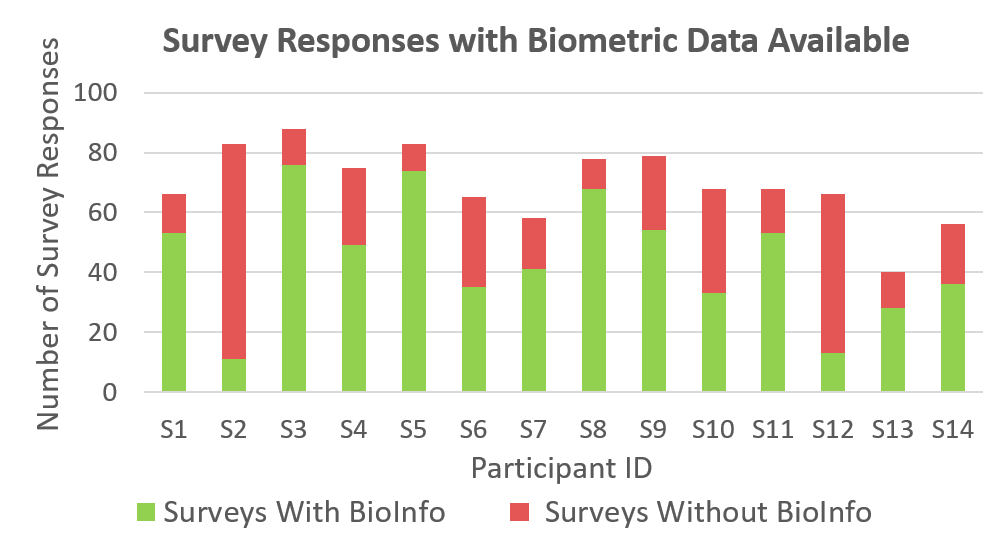
\includegraphics[width=0.8\textwidth]{DuringTheDay.png}
  \caption{The figure shows the biometric data available per each participant. Green sections represent survey responses with biometric
  data available, red sections responses with no biometric data available}
   \label{surveyBio}
   \vspace*{-4mm}
\end{figure}


\subsubsection{Feature Extraction}
We extracted features from the biometric data to provide as input to machine 
learning models. Previous 
studies~ \cite{vorburger05,zuger2015interruptibility} identify time windows as an 
important factor that impacts the prediction accuracy of a classifier. We 
considered many time windows from the literature on biometric 
analysis~\cite{zuger18}, ranging from 10 seconds to 3 hours. Specifically, we 
considered the following time windows: \textit{10sec, 20sec, 30sec, 45sec, 
1min, 2min, 3min, 5min, 7.5min, 10min, 20min, 30min, 45min, 1hour, 2hour, 
3hour}.

From the start time of each survey response, we look back the amount of time 
that corresponds to each time window and we create features for all of the 
biometric data available in that time window. For example, if a participant 
started a survey response at 11:05am, for the 30min time window, we create 
features using all of the available biometric data from 10:35am to 11:05am. 
If there is a large portion ($\geq$50\%) of data missing (either because of a recording issue or because of low quality data) from the time window considered, then the time window is marked as missing. In this case, features are imputed based on the mean of other samples of the same feature for that participant. This is an effective and commonly used technique, which is preferable to the alternative of deletion as it preserves our already small sample size~\cite{hawthorne2005imputing}.
For each time window, we calculate 10 statistical measurements from the 
biometric data to create 10 distinct features. Specifically, the 10 
statistical measurements are: mean, standard deviation, variance, median, 
25\textsuperscript{th} percentile, 75\textsuperscript{th} percentile, interquartile range, maximum, minimum, and 
range. Thus, for each survey response, we generate a large number of 
corresponding features based on three factors: biometric measurement, time 
window, and statistical measurement. In addition to these biometric 
features, we also considered the time of day in which the questions were 
asked. These features are created to predict the responses described by the 
ground truth. To attempt to account for inter-participant differences, we normalized all features on a per-participant basis.

\begin{table}
  \centering
      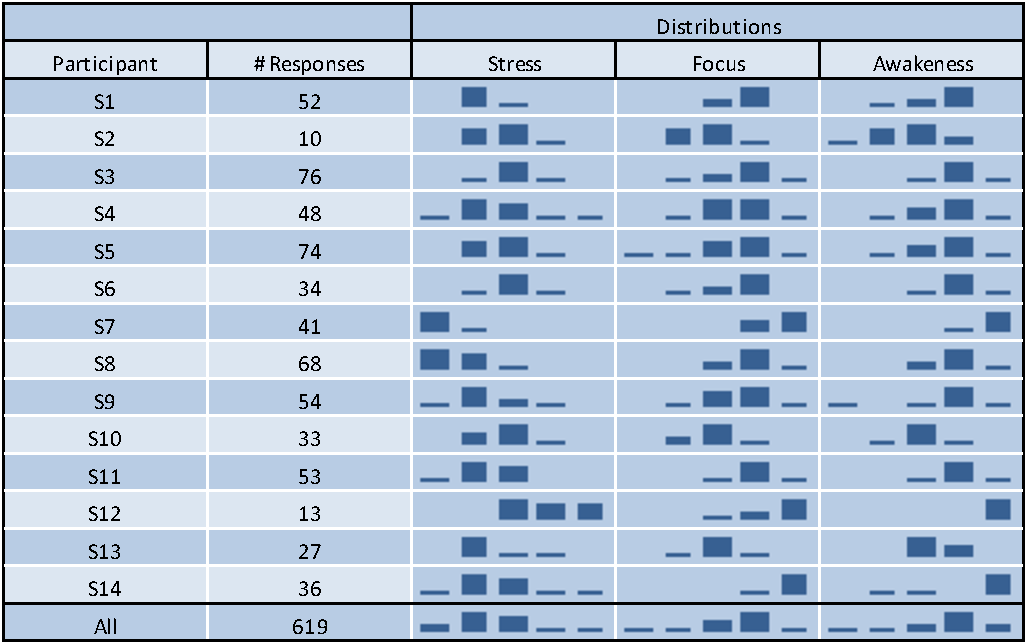
\includegraphics[width=0.8\textwidth]{distributiontable.pdf}
  \caption{The distribution of the responses of each participant to the three questions asked during the day are shown. Each bar in the histograms represent one of the \ref{five} values on the 5-point Likert scale we asked participants to respond with, where the far left side of the histograms are 1/Not at all, and the far right sides are 5/Extremely}
   \label{responseDistribution}
   %\vspace*{-2mm}
\end{table}

\subsubsection{Response Transformations}
Table~\ref{responseDistribution} illustrates the distribution of responses from each participant for each of the three survey questions (listed in Section~\ref{sec:Surveys}). The figure shows that there is a notable imbalance in the distribution of the self-reported responses provided by the participants. Most participants did not use all five points of the five-point Likert scale in their responses, and the distributions tend to skew toward one side or the other, depending on the question. Given 
this distribution and based on our earlier observation that the participants tended to adhere to a baseline reporting level for stress and awakeness, we elected to simplify the problem from \rev{five} classes to \rev{two}. This transformation enables us to more easily represent patterns in the data, such as when a participant fluctuates from a normal to high stress level. To perform this transformation, \rev{we began by calculating the median response value for each participant and each question}. We classified each response below the median as 0 (`negative') and each response above the median as 1 (`positive'). The distribution for the stress question skewed left, so we included the median values in the `positive' class (i.e. `stressed'), while the distributions for focus and awakeness skewed right, so we included those median values in the `negative' class (i.e. `not focused', `not awake').

With this method, we transformed the survey data into a two-point scale, representing  negative or positive responses for each of the three human aspects of interests (e.g., not stressed or stressed). 

\subsubsection{Oversampling}
Even after binarizing the responses as described in the previous section, we found the distribution of responses was still quite imbalanced for many of our participants. This can be seen in the distribution columns in Table \ref{tab:accuracy}. To mitigate this effect, we applied random oversampling to our training sets, which artificially rebalances the dataset by creating randomly replicated data in the minority class. This technique has commonly been used  in previous studies on unbalanced datasets \cite{chawla2004,yap2014}.

\begin{comment}
\begin{table}[h]
	\begin{centering}
	\small\addtolength{\tabcolsep}{-1pt}
    \begin{tabular}{llll}
      \hline
      Variable & K & \# Estimators & Minimum Samples Split \\
      \hline
      Stress & 300 & 100 & 4\\
      Focus & 200 & 50 & 4\\
      Awakeness & 800 & 100 & 4\\
      \hline
    \end{tabular}
    \caption{The hyperparameters selected by grid search analysis to tune our random forest models. K refers to the number of features selected.}    \label{tab:hyperparams}
    \end{centering}
\end{table}
\end{comment}


\subsection{Selecting a Classifier Algorithm}

\rev{Many different algorithms can be used to build a classifier.} To select an
algorithm, we compared multiple classifiers using the popular machine learning library scikit-learn~\cite{pedregosa11},  evaluating each one by using leave-one-out cross validation. Our analysis showed that random forest outperforms all other classifiers, including Na\"ive Bayes, decision trees, support vector machine, and a multilayer perceptron neural network. For the remainder of this paper, we refer to a random forest classifier.%\\[-0.1cm]
% for stress they were (minimum samples for split = 4, # of estimators = 100, max features = 0.5, k=300), for focus they were (minimum samples for split = 4, # of estimators = 50, max features = 0.5, k=200), and for awakeness they were (minimum samples for split = 4, # of estimators = 100, max features = 0.25, k=800)



\begin{table*}[h]
  \centering
  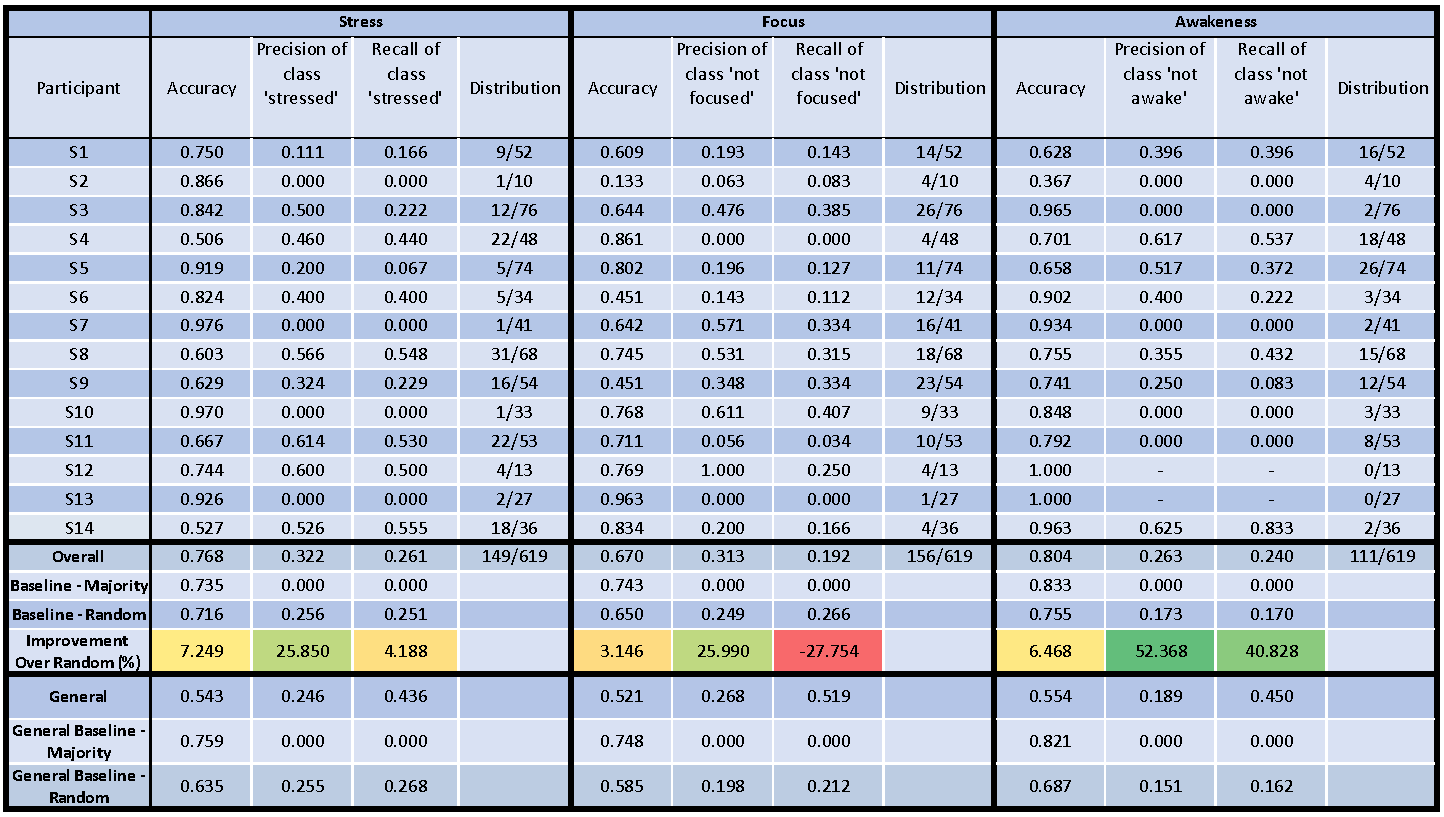
\includegraphics[width=1.0\textwidth]{rq1performance_v2.pdf}
  \caption{Results of predictions using the individual models. The distribution columns show the proportion of the minority class out of the total number of responses for each of the three variables. The baseline rows represents the averaged results of our baseline classifiers. The general row shows the averaged results of our models trained on all participants.}\label{tab:accuracy}%\todo{revise caption}}
  \vspace*{-4mm}
\end{table*}

\subsection{Individual Classifiers}
%\noindent\textit{Results of Individual Classifiers}\\
Since peoples' experience of stress, focus, and awakeness (as well as
their physiological manifestations) can vary substantially
(e.g.,~\cite{Hernandez11}), we first trained and evaluated individual classifiers
for each participant (as opposed to a general one for all
participants) using leave-one-out cross validation. The results of our analysis are reported in
Table~\ref{tab:accuracy}. For our analysis, we report values of
accuracy, one of the most commonly used metric to compare performance,
as well as precision and recall of the classes of interest:
`stressed', `not focused', and `not awake'. Since the imbalance in the
data can lead to high accuracy values if a classifier always just
predicts the most likely/frequent class while ignoring the class of
higher importance and interest, precision and recall of the class of
interest are also important to
consider~\cite{yap2014,bhattacharyya_data_2011,Hernandez11}.

\rev{Besides} our results, for the purposes of comparison\rev{,} we also present two commonly used baselines in this table - a majority classifier, which always predicts the larger of the two classes considered, and a stratified random classifier which randomly chooses between the two classes, but with a proportional bias towards the larger class.

For some users (i.e., S1. as seen in Table \ref{responseDistribution}), the imbalance in their data was so extreme that even after adjusting by oversampling\rev{, we were not able} to create a reasonable classifier. These scenarios are difficult to predict\rev{,} as any classifier will not have enough variance in its training data for the 'stressed' situation to adequately distinguish it from the non-stressed case.


% However, the imbalance in the data can lead to a classifier with high accuracy if it always just predicts the more likely class while ignoring the class of higher importance and interest in our case (i.e. stressed, not focused, not awake). Therefore, we further report the precision and recall for the three classes 'stressed', 'not focused' and 'not awake'. 


Overall, we were able to use extracted physiological features to
predict all three aspects with reasonable accuracy, precision, and
recall. We present a comparison between the averaged results of our individual classifiers and those of the baseline stratified random \rev{classifier} in the ``Improvement Over Random'' row of Table \ref{tab:accuracy}. This is calculated as the difference between the overall average and the baseline results, divided by the baseline results (for example, $\frac{Acc_{Overall} - Acc_{Random}}{Acc_{Random}}$). We do not compare our results with the majority classifier directly as this classifier achieved precision and recall scores of zero when predicting stress, lack of focus, and lack of awakeness, making a meaningful comparison \rev{unfeasible}. The improvement percentages demonstrate that the predictions made by our classifiers are much better than random after correcting for the imbalance in our dataset.

While the individually trained classifiers
improved on average across all participants upon the baseline in all
cases except in recall of `not focused', the improvement was
substantially higher for awakeness (52.4\% improvement in precision,
40.8\% in recall, and 6.5\% in accuracy) than for stress or focus. In addition,
the performance of the individually trained classifiers varied greatly
across participants. While some participants showed a large
improvement, for others the baseline performed much better than the
individually trained classifier. For instance, for predicting
`stressed', the individual classifiers improved upon the baseline for
S4, S6, S8, S11, S12, and S14 with a maximum improvement of 152.0\% in
precision and 111.1\% in recall for S12, while they did worse for S1,
S3, S5, S7, S9, S10, and S13, and in the worst cases did not correctly
predict a single instance of `stressed'. Typically, users that have the
lowest precision and recall values are those where the data is the
most imbalanced.\\[-0.1cm]
% We attribute these discrepancies to the large differences in response distributions between participants, as well as to the subjectivity of self-reporting.
%
%(improvement: 8\% precision, 1\% recall, 8\% accuracy), the individual performance varied greatly among participants. Some participants showed negligible difference in comparison to the baseline classifier, e.g. subject ..., while others showed a large improvement, e.g. subject ...
%\begin{table}[h!]
%\begin{centering}
%\begin{tabular}{lll}
%\hline
%Participant & Recall Improvement (\%) & Precision Improvement (\%)\\
%\hline
%S12 & 184.6 & 88.4 \\
%S6 & 66.7 & 85.8 \\
%S11 & 50.0 & 44.4 \\
%S8 & 32.4 & 26.7 \\
%S14 & 14.7 & 9.8 \\
%S4 & 5.6 & 5.5 \\
%S9 & -55.4 & -46.8 \\
%S3 & -90.0 & -82.1 \\
%S1 & -100.0 & -100.0 \\
%S5 & -100.0 & -100.0 \\
%S7 & -100.0 & -100.0 \\
%S10 & -100.0 & -100.0 \\
%S13 & -100.0 & -100.0\\
%S2 & - & -\\
%\hline
%\end{tabular}
%\caption{Percentage improvement in recall and precision for stress, using our approach compared to the baseline, on an individual level. For participant 2, the baseline achieved a precision and recall of 0, thus the improvement is undefined}
%\end{centering}
%\label{tab:indImprovement}
%\end{table}


\subsection{Feature Selection and Importance}
%\noindent\textit{Feature Selection and Importance}\\
There are a large variety of features that can be (and have been) calculated in previous research for each of the basic measurements listed in Table~\ref{signals}, such as the mean, standard deviation, maximum, and interquartile range. In addition, each of these metrics can be combined with the various time windows captured of a basic measurement, resulting in a large feature space. To reduce the feature space, we experimented with multiple feature selection methods, including selecting the top k highest correlated features by various metrics such as mutual information, Pearson's correlation coefficient, ANOVA's F-value, as well as wrapper methods such as recursive feature elimination, optimizing mean decrease accuracy by iteratively permuting features, and only selecting features that exceed a certain Gini importance threshold. We found that all methods produced similar results with respect to accuracy, precision, and recall for the individual models. Ultimately, we elected not to utilize any feature selection in order to simplify our approach, as we found there to be minimal differences in performance between the techniques, and the random forest algorithm is capable of (and robust for) handling datasets with many features.

%Respiration rate is also highly important for stress (#3 , 14.4%) but I'm not sure what previous works say about correlation with stress
Overall, the features that were selected as the important ones for the individual models based on the random forest algorithm varied greatly across participants. Yet, some feature categories were considered to be important more frequently than others. Table~\ref{tab:featureImportance} shows the averaged Gini importance for the feature categories used for predicting stress. Heart rate variability proved to be an important measure for all of the aspects of interest, ranking as the most important feature category for both stress and awakeness, and the second most important one for focus. This is not surprising, as heart rate variability and skin temperature have been shown in several previous studies to be possible indicators for stress levels~\cite{dishman2000stress,mcduff16,kataoka00}. We also found blood pulse wave to be an important indicator for both focus and awakeness, but less important for stress, while respiration rate was important in stress and focus but not awakeness. Besides these mentioned feature categories, there was great variation in which measures were important to which of the three aspects. This shows that there is a clear benefit to having multiple biometric streams available for predicting stress, focus and awakeness.\\[-0.1cm]


\begin{table}[h!]
  \begin{centering}
  \begin{tabular}{llll}
    \hline
    Feature Category & Stress & Focus & Awakeness\\
    \hline
    Heart Rate Variability & 18.3\% & 13\% & 13.6\%\\
    Blood Pulse Wave & 10\% & 14.2\% & 13.1\%\\
    Heart Rate & 8.7\% & 12.6\% & 10.3\%\\
    Skin Temperature & 15.7\% & 9.8\% & 10\%\\
    Galvanic Skin Response & 6.6\% & 8.2\% & 5.1\%\\
    Respiration Rate & 14.8\% & 12.7\% & 10\%\\
    Oxygen Saturation & 5.6\% & 4.3\% & 2\%\\ 
    Energy Expenditure & 6\% & 7.7\% & 4.8\%\\
    Activity & 4.6\% & 7.8\% & 7.6\%\\
    Steps & 1.7\% & 0.8\% & 0.9\%\\
    Time of Day & 0\% & 0.1\% & 0.5\%\\
    \hline
  \end{tabular}
  \caption{The averaged Gini importance of each feature category, per response variable.}
  \label{tab:featureImportance}
  \end{centering}
  \vspace*{-2mm}
\end{table}

\subsection{Individual vs.\ General Model}
%\noindent\textit{Individual vs.\ General Model}\\
Individual models are trained specifically for each individual and thus require a data collection period before they are capable of making accurate predictions. On the other hand, the idea of general models is to be able to train them on already collected data and then  to be able to apply them even to new and unseen individuals, thus overcoming the cold-start problem. Given the large individual differences in biometrics, training a general model to achieve an adequate accuracy for new individuals is not necessarily possible. 

To examine the performance of a general model for our participants, we trained three general models, one for focus, one for awakeness and one for stress. We roughly followed the same procedure as for the individual models. Due to the larger amount of data available in the general case, we used the more common random undersampling, which randomly selects elements in the majority class to exclude from the dataset, instead of random oversampling to balance the distribution of the dataset. The models were trained on the datasets of 13 of the 14 participants, and then evaluated on the dataset of the last (leave-one-participant-out cross-validation), repeating this process for all 14 participants. 

The bottom \rev{three} rows of Table \ref{tab:accuracy} present the averaged performance results for this approach in terms of accuracy, precision, and recall, as well as the results of baseline stratified random and majority classifiers following the same leave-one-group-out cross-validation procedure. Although the averaged precision and recall are comparable or better than those of the averaged individual results, this was at the cost of a large decrease in overall accuracy.  Upon closer investigation into the performance of the general model when testing on each participant, we found that individually trained models for each participant performed much better than a general model trained over all participants. Using stress as an example, for participant S12, for whom we saw the greatest increase compared to the baseline in individual models, the general model was unable to predict a single instance of `stressed' correctly. This is consistent with our expectations because biometric features are highly specific to individuals.


%\todo{put the content of the following sentence somewhere into the discussion; We attribute these discrepancies to the large differences in response distributions between participants, as well as to the subjectivity of self-reporting.}


%%%!TEX root = bioPrediction_main.tex

\subsection{Minimum Number of Training Samples}\label{secLearningCurve}
Collecting experience samples from users is expensive, since participants 
are being interrupted several times a day and have to answer the survey. 
To minimize the number of samples to be collected from participants, we 
examined how the performance of individual classifiers changes over the 
number of samples used to train the classifier.

Participants in our study had varying levels of responsiveness to the 
experience sampling ranging from 10 to 76 (see Figure~
\ref{responseDistribution}).
%Answering Reviewer 2's concern: Why only 10 participants? What was the rationale for the cut-off selected? 
To answer this research question we analyze the maximum number of responses \textbf{all} analyzed participants have to train the model. Since some participants have a very small number of maximum answers (ten being the lowest) we excluded the four participants with the least number of responses for this analysis.
%To maintain a certain generalizability while 
%also being able to examine a range of sample numbers for training the 
%classifier, we removed the four participants with the least number of 
%samples for this analysis. 
As a result, we obtained a corpus of analysis where all participants have a 
higher number of responses (34 being the lowest), which allows us to examine 
the learning curve of the classifiers for a larger number of training data points. For our 
analysis, we thus performed a leave-one-out cross validation with random 
sample sets of size 1 to 33 and calculated the average through all folds of 
the validation.

For each of the three productivity-related aspects, we are again more 
interested in predicting when a worker is stressed, not awake, or not 
focused, the less common class in all three cases. Since the less common 
class can be very small, we weighted each participants' classifier 
performance by the percentage of the samples in this smaller class.

\begin{figure}
  \centering
          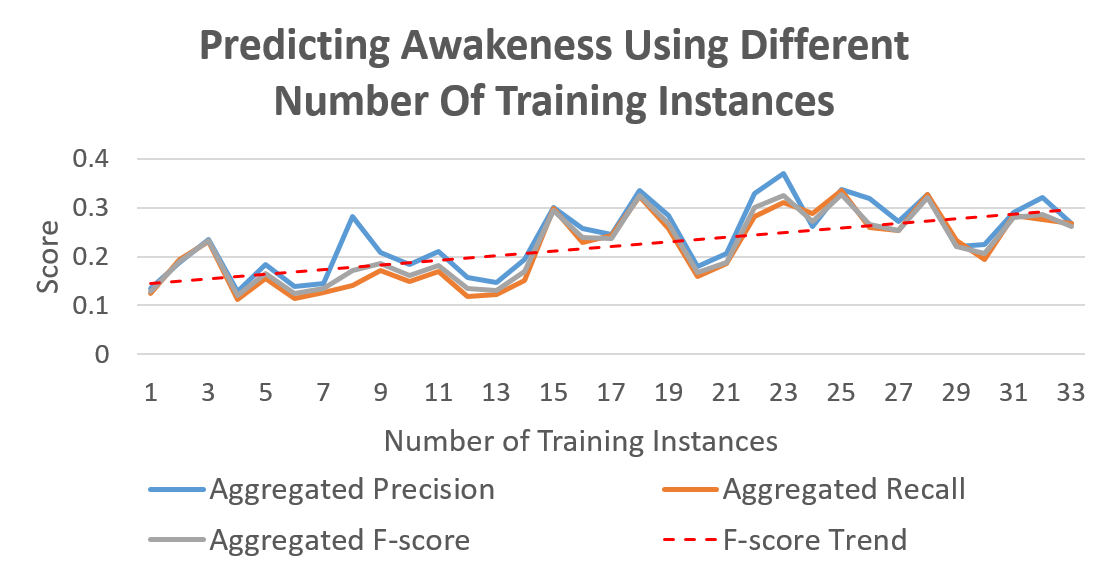
\includegraphics[width=0.5\textwidth]{20180912AwakenessLC2.png}
  \caption{Performance of the per participant trained awakeness classifiers, measured in precision, recall (sensitivity), and F-score. The dotted red line represents the F-score trend.}\label{fig:learningCurveInd}
  %\vspace*{-3mm}
\end{figure}

%\vspace{0.05in}
\noindent\textit{Individual Classifiers for Binary Prediction}\\
The averaged performance of all individually trained random forest classifiers for 'awake' with respect to the training sample size is presented in Figure~\ref{fig:learningCurveInd}. The trend indicates a positive correlation between the number of samples in the training set and the classifiers' F-score performance, with an overall improvement of  114\% (from 0.14 to 0.30) in the F-score between a training set of one sample to one with 33 samples. The trends for
the remaining indicators are 29\% for stress and no overall improvement for focus.%\\[-0.1cm]

%\noindent\textit{}
%When contrasting
%models trained and tested on the 
%biometric data of each user individually, against
%a general model trained and tested with the data of all users. 
%We can conclude
%that for up to 33 training samples analyzed in this study,
%the former has better performance when predicting the
%responses of each user than when training 
%a model with the data of several different users. 
%This is partially due to the 
%variability across users and the subjective nature
%of the responses (e.g.,where slightly awake for one person
%may be not awake for another). 

\begin{figure}
  \centering
      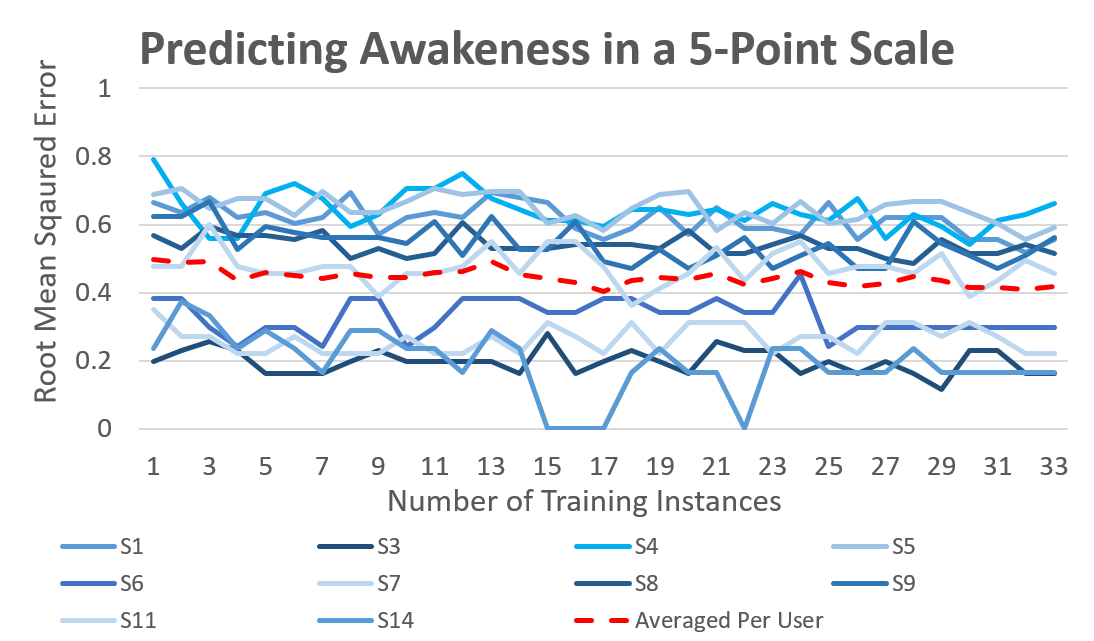
\includegraphics[width=0.5\textwidth]{20180914Awakeness5PointScaleOnly15Lines.png}
  \caption{Performance of the per participant trained classifiers for predicting 5-point awakeness, measured in root mean squared error.}
   \label{fig:learningCurve5}
\end{figure}

\noindent\textit{Predicting Five Classes}\\
In a second step, we analyzed a more fine-grained prediction using the initial 5-point Likert scale responses rather than the binarized ones as output measure. Figure~\ref{fig:learningCurve5} depicts the performance of the individually trained classifiers in terms of the root mean squared error. The root mean squared error represents the distance of the predicted from the actual value, which provides a more nuanced measure of the performance in the fine-grained prediction case. The figure shows a similar trend as for the binarized prediction, in that the root mean square error averaged over all ten participants decreases with more samples (from 0.49 to 0.41 root mean square error) and thus the performance increases. At the same time, the figure also shows that the performance results for the fine-grained prediction, again, vary substantially across participants.

\subsection{Minimum Time Window}\label{secMinimumTW}
In general, the less biometric data is needed to accurately predict a certain outcome measure, the easier and faster the analysis and data collection. To examine the optimal and minimum time window for the prediction of stress, focus, and awakeness, we used 16 different time windows from 10 seconds to 3 hours as depicted in Figure~\ref{timeWindows}. For our analysis, we then trained individual classifiers for each of the 16 time windows, using only features that had a time window smaller or equal to the time window rather than using all combinations of $\{Biometric Measures\} X \{Statistical Metrics\} X \{Time Windows\}$. We again used random forest and a leave-one-out cross validation to train individual classifiers. Since the number of features used for the training changed with each time window, we did not apply our feature selection in this case, but used all features available. Finally, due to the imbalance in the data, we again weighted each participants' classifier performance by the number of instances in the smaller class to calculate the average.

\begin{figure}
  \centering
      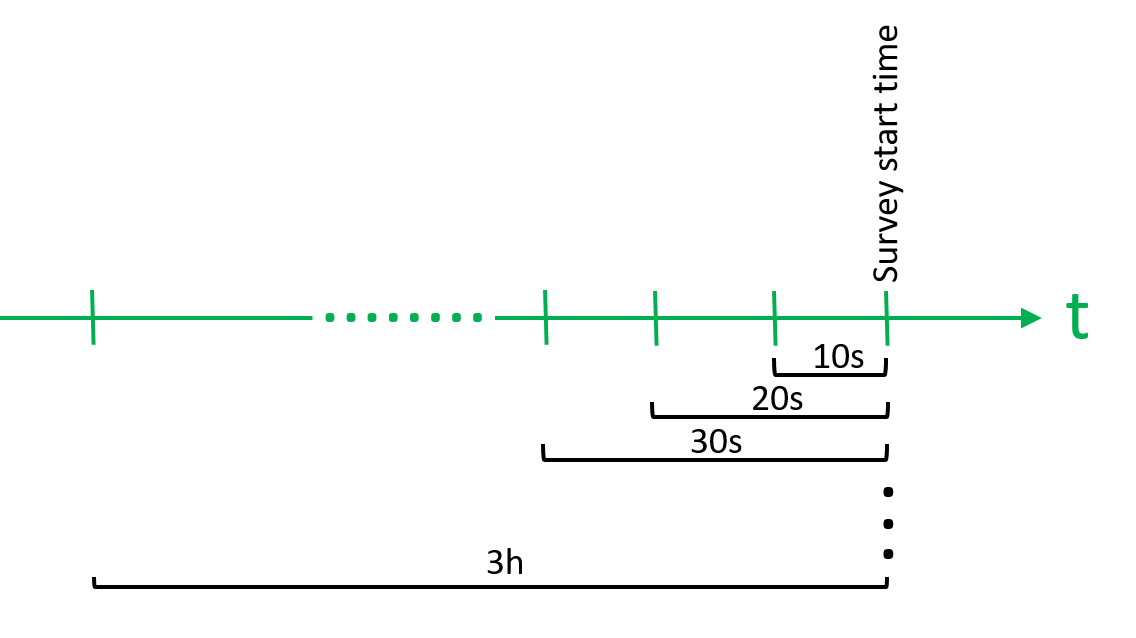
\includegraphics[width=0.4\textwidth]{timeWindows.png}
  \caption{Time windows of biometric data collected prior to each survey response: 10sec, 20sec, 30sec, 45sec, 1min, 2min, 3min, 5min, 7.5min, 10min, 20min, 30min, 45min, 1hour, 2hour, and 3hour.}
   \label{timeWindows}
\end{figure}

Figure~\ref{timeWindowsPandR} shows how the F-score changes for predicting 
`awake' over the 16 different time windows. The figure shows an increasing 
trend in the F-score, i.e. the higher the number of included time windows, 
the higher the F-score. However, there is one exception, the time window of 
1200 seconds that achieves a performance close to the one for the time 
window 10,800 seconds (3 hours), at which point all features are included. 
Overall, our results thus show that while using all time windows up to 3 
hours performs best, and outperforms the feature set that is solely based on 
a 10 second time window by 28\% (from 0.18 to 0.24), the performance for a 
time window of 1200 seconds is a good trade-off for selecting a shorter time 
window while maintaining high performance.

\begin{figure}
  \centering
      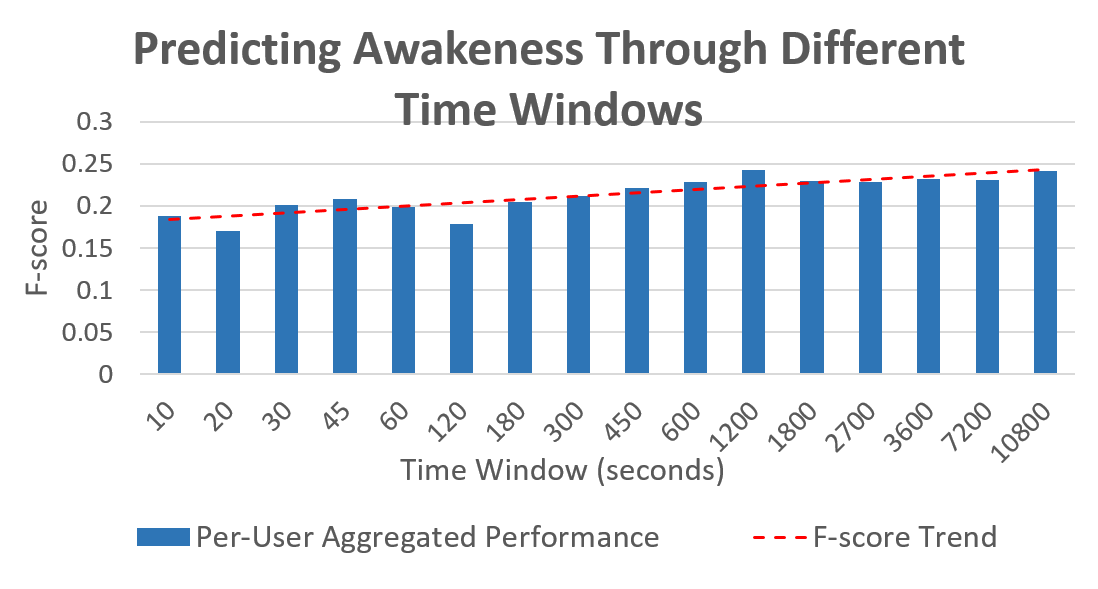
\includegraphics[width=0.5\textwidth]{20180912AwakenessTWBars.png}
  \caption{Performance (F-score) of individual classifiers trained on the different time windows to predict `awake'.}
  \label{timeWindowsPandR}
 % \vspace*{-3mm}
\end{figure}

%We also compared the performance of a model created per user against
%a model created across users.
%To calculate the performance of the model created per user,
%for each user we create a model using the features 
%related to each time window for the selected user only, 
%while in the model created with data across users,
%we trained the model with the data related to each
%particular time window of all users.
%our results show that the personalized model created
%for each user outperforms in every case
%the model created the with data across all users.

%This study
%shows that in general larger time windows predict stress,
%focus, and awakeness more precisely than 
%shorter time windows. We can also notice
%a very gentle upwards trend
%with a inflexion points at 45 seconds and 180.
%There is a peak of performance in 45 seconds, 
%time window that could be used if time is a scarce resource.
%The performance stabilizes around 180 time window
%which indicates that collecting data for a longer time
%period will not increase significantly the performance of the approach.
%The difference in performance between the 
%lowest performing and the highest performing time window is 
%less than a 10\% improvement. 


\subsection{Computer Interaction Data} \label{secCI}
Given our focus on knowledge workers (i.e., workers who generally spend a lot of time interacting with information on their computer at work), we also analyzed the use of computer interaction features to predict focus, awakeness and stress. To collect computer interaction data, we used an open source computer interaction monitor (reference omitted for double-blind.)
%the open source PersonalAnalytics project\footnote{https://github.com/sealuzh/PersonalAnalytics}  \cite{meyer18} 
to track participant's mouse and keyboard activity, as well as details about their active window. The specifics of the features tracked are listed in Table \ref{tracker}. The tracker was installed on the computers of 10 of the 14 participants, with participants S6, S10, S12, and S13 opting out of this part of the study due to privacy concerns.  Therefore, we limited this analysis to the 10 participants for whom we could calculate all features. 

\begin{table}
\begin{center}
\small\addtolength{\tabcolsep}{-1pt}
\begin{tabular}{l l}
\hline

Feature collected by tool & Description \\ 
\hline
Total keystrokes per min& Sum of all types of keystrokes \\ 
Normal keystrokes per min&F[h] Not backspace and navigation \\ 
Backspace keystrokes per min& Backspace keystrokes \\ 
Navigation keystrokes per min& Arrow key keystrokes \\ 
Total clicks per min& Sum of all click types \\ 
Other clicks per min& Not right and left clicks \\ 
Left clicks per min& Left clicks \\ 
Right clicks per min& Right clicks \\ 
Scrolled distance per min& Scrolled distance in pixels \\ 
Moved distance per min& Mouse movements in pixels \\ 
Activity switches per min& Browser window title changes \\ 
Category switches per min& Activity performed category \\ 
\hline
\end{tabular}
\caption{Features collected per user by the computer interaction tracker}%~\cite{meyer18}}
\label{tracker}
\end{center}
%\vspace*{-1mm}
\end{table}

For calculating computer interaction features, we again used the aforementioned 16 time windows and scaled the computer interaction values if the time windows did not align. For our comparative analysis of the different sensing techniques---biometrics vs computer interaction---we then created two new feature sets for each participant in addition to the biometric one: one with only computer interaction features, and one with computer interaction features plus biometric features. 

Table~\ref{ciPerformance} lists the results of our analysis. The results show that in all cases, the computer interaction based model was able to improve upon the biometric model in terms of precision and recall.
%MS is removing the accuracy results because it is not what we care about and it is just making the results harder to understand
%, but not in accuracy. 
Further, we found that the combined model was the most effective model in terms of precision and recall for predicting stress and awakeness overall, but performed slightly worse than the model using only computer interaction features for focus. 
%Since we consider precision and recall for predicting the class of higher interest, i.e. stressed, not focused, not awake, to be the most important statistics when interpreting our results, we compared the models against each other by averaging these two statistics.


\begin{table}
\begin{center}
%\small\addtolength{\tabcolsep}{-1pt}
\begin{tabular}{llllll}
\hline
Model/Feature Set & Precision & Recall & F-Score \\ %& Accuracy\\
\hline
\textbf{Awakeness}\\
\hspace{3mm}Biometrics only  & 0.269 & 0.314 & 0.289 \\ %& 0.808\\
\hspace{3mm}C.I. only  & 0.425 & 0.362 & 0.391 \\ % & 0.758\\
\hspace{3mm}Biometrics + C.I. & 0.390 & 0.404 & 0.400 \\ % & 0.791 \\
\hline
\textbf{Stress}\\
\hspace{3mm}Biometrics only  & 0.270 &	0.260 & 0.265 \\ % & 0.775\\
\hspace{3mm}C.I. only & 0.290 & 0.272 & 0.281 \\ % & 0.698 \\
\hspace{3mm}Biometrics + C.I. & 0.317 & 0.286 & 0.301 \\ % & 0.712\\
\hline
\textbf{Focus}\\
\hspace{3mm}Biometrics only & 0.251 & 0.256 & 0.253 \\ % & 0.716\\
\hspace{3mm}C.I. only & 0.332 & 0.342 & 0.337 \\ % & 0.742\\
\hspace{3mm}Biometrics + C.I. & 0.340 & 0.316 & 0.328 \\ % & 0.745\\
\hline
\end{tabular}
\caption{Comparison of the performance of predicting stress, focus and awakeness using the 3 different feature sets for the 10 participants. The performance is calculated as the average of the performance of the individual classifiers. Computer Interactions is abbreviated as C.I. here for readability. Precision and recall refer to the prediction of the more important classes, i.e. `stressed', `not awake', `not focused'.}
\label{ciPerformance}
\end{center}
%\vspace*{-1mm}
\end{table}

As with the biometric models, the individual performance of both the computer interaction only models and the combined models varied quite a bit between participants. Using stress as an example again, in the computer interaction models 5 of the 10 participants saw improvements compared to the baseline, with a maximum improvement of 128\% in precision, and 78\% in recall. In the combined model for stress, 5 of the 10 participants saw improvements compared to the baseline, with a maximum improvement of 117\% in precision and 95\% in recall. Neither model was capable of correctly predicting any instances of 'stressed' for participant S7.

Since the number of features changes  depending on which feature set is used, we adjusted the feature selection parameter for each of the computer interaction and combined computer interaction/biometric models. The values reported in this section were achieved using the optimal feature selection parameters we found, which are shown in Table \ref{ciFeatureSelection}.

\begin{table}
\begin{center}
\begin{tabular}{lc}
\hline
Model/Feature Set & Number of Features Selected\\
\hline
\textbf{Stress}\\
\hspace{3mm}C.I. & 400\\
\hspace{3mm}Biometrics + C.I. & 800\\
\hline
\textbf{Focus}\\
\hspace{3mm}C.I. & 20\\
\hspace{3mm}Biometrics + C.I. & 300\\
\hline
\textbf{Awakeness}\\
\hspace{3mm}C.I. & All\\
\hspace{3mm}Biometrics + C.I. & 50\\
\hline
\end{tabular}
\caption{The optimal number of features we found to select for each of the model/feature set combinations. Computer interactions is abbreviated as C.I.}
\label{ciFeatureSelection}
\end{center}
\vspace*{-4mm}
\end{table}



%\section{Analysis and Results}

\begin{table*}[h]
  \centering
  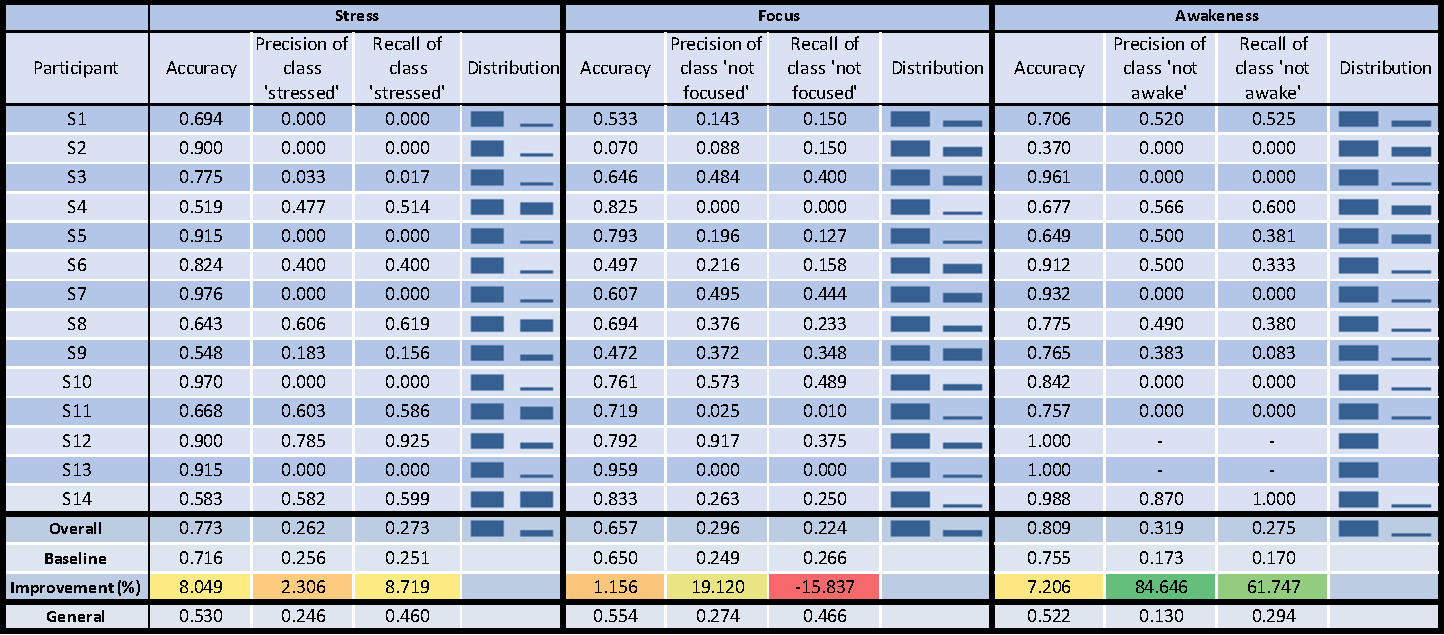
\includegraphics[width=1.0\textwidth]{rq1performance.pdf}
  \caption{Results of predictions using the individual models. The distribution columns show a bar chart of the response distribution (negative/positive) for each of the three variables. The baseline row represents the averaged results of our baesline classifier. The general row shows the averaged results of our models trained on all participants.}\label{tab:accuracy}%\todo{revise caption}}
  \vspace*{-4mm}
\end{table*}

%% To evaluate the efficacy of continuously predicting a knowledge worker's stress, focus, and awakeness in the workplace, we trained and tested machine learning classifiers using a leave-one-out cross validation. For prediction, we used the features extracted from the collected data as the input data, and binarized the participants' self-reported responses on stress, focus, and awakeness into two classes each (e.g., 'stressed' and 'not stressed') to use as output measures.

\section{Observed Trends Over Time in Stress Levels}
\label{stressTrends}

To gain insights into how knowledge workers experience stress over an
extended period of work, we examined the end of day survey responses
collected from each participant to see if any identifiable trends
emerged. We used data from 13 of the 14 participants - we excluded one participant
from this analysis as they experienced atypical stress
levels in the latter half of the study due to factors outside of our
control.

\subsection{Baseline Stress Levels}
Common amongst all participants was a trend to select one stress rating
far more frequently than any other. We will refer to this value as the
participant's baseline stress level. All but one participant reported
their perceived stress level for the day as their baseline stress
level more than 50\% of the time. In total, the baseline values made
up 65\% of the reported values collected from
participants. Interestingly, while participants sometimes saw periods
of sustained increases in stress, lasting as many as 6 consecutive
workdays in the most extreme case, participants would always return to
their baseline stress level at some point.

\begin{figure}
  \centering
      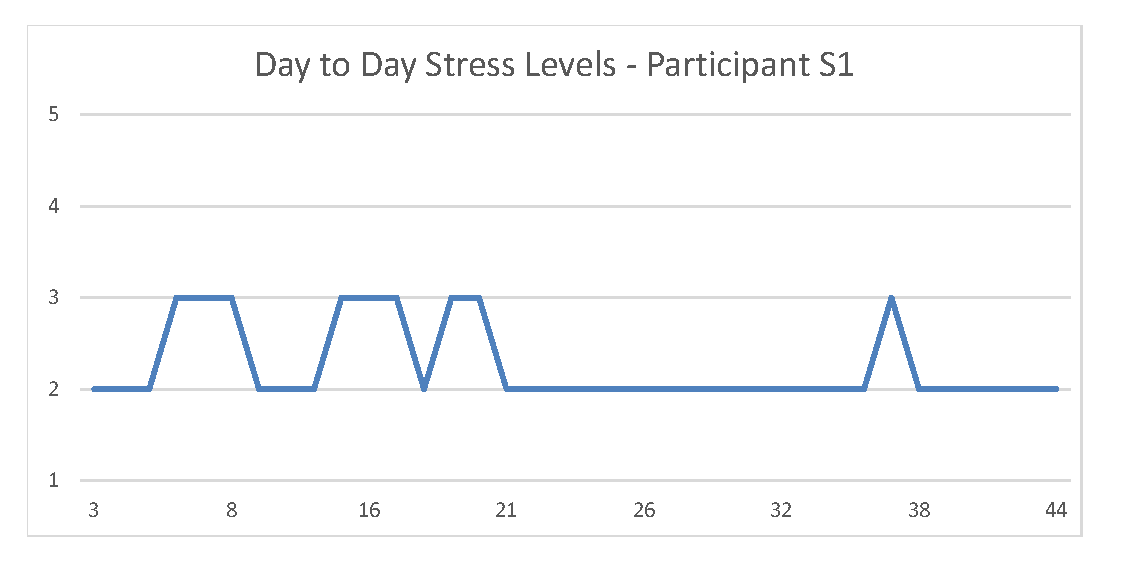
\includegraphics[width=0.5\textwidth]{dailystress_s1.pdf}
      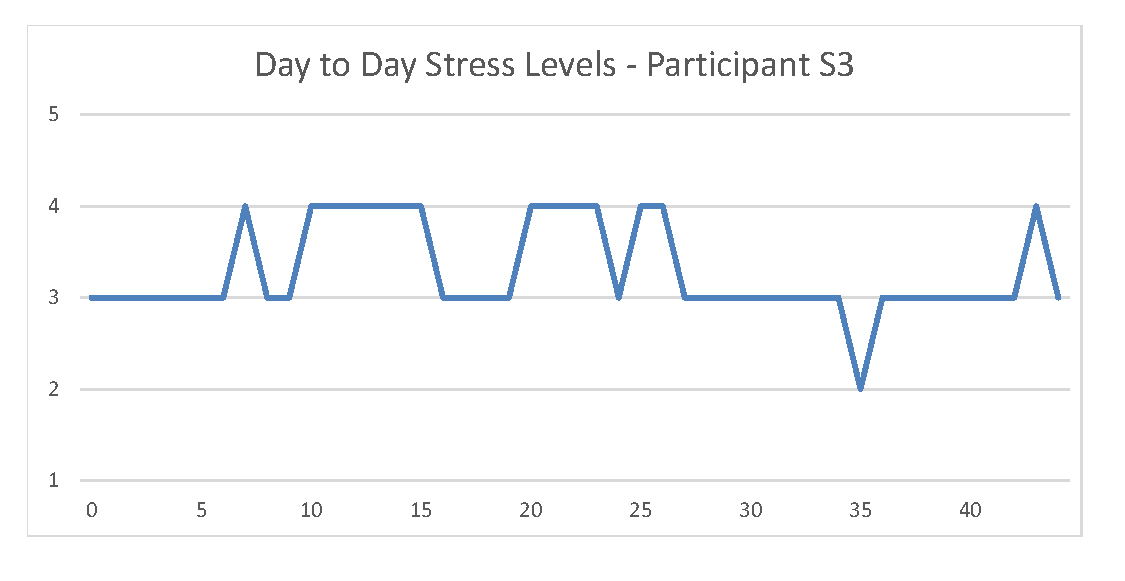
\includegraphics[width=0.5\textwidth]{dailystress_s3.pdf}
  \caption{The day-to-day stress levels reported by two participants (S1 and S3) are shown. The y-axis represents values on the 5-point Likert scale we asked participants to respond with ranging from 1/Not at all stressed to 5/Extremely stressed. The x-axis represents the day of the study on which the value was recorded (from 0-45). The x-axes are slightly different for the 2 participants as they did not begin and end the study on exactly the same days.}
   \vspace*{-2mm}
   \label{fig:dailyStress}
\end{figure}

The baseline stress level varied significantly between participants. 7
participants (54\%) reported feeling average stress levels most frequently
(rating 3 on our scale), while 5 (38\%) reported feeling little stress
(rating 2) and 1 (8\%) reported feeling no stress at all (rating 1).

Figure \ref{fig:dailyStress} illustrates these points, showing both participants tendency to report and return to baseline stress levels

\subsection{Stressful Days Tend to Cluster}
Accounting for the variance between participants perceived stress
baselines, we consider a stressful day to be one that represents a
deviation of 1 or more stress levels above the participant's
baseline. Of the 93 stressful days we observed in total, we found that
39 (41\%) of these days occurred in groupings of two or more
consecutive stressful workdays. The most common size of these groups
was two workdays, while the largest group we observed was six
workdays.  The day after a stressful day is much more likely to be a
stressful day as compared to any other day with a 0.55 average increase
over baseline, compared to 0.02 average increase over baseline.

\subsection{Extreme Changes in Stress Levels are Rare}
After accounting for each participant's perceived stress baseline, we
examined the frequency of deviations from the baseline. We found that
participants were far more likely to report a stress level that was
within 1 point of their baseline, than to report a stress level 2 or
more points away. These extreme deviations represented only 15\% of
all reported values which differed from the participants baseline. As
well, the majority (78\%) of these deviations came from just two
participants. This suggests that some people may be less resilient to
the stress of the workplace than others. For most participants,
extremely stressful days were few and far between.

\subsection{Explaining Stress Fluctuations}
We created a linear mixed model to attempt to explain some of the
stress that our participants were experiencing. We experimented with
multiple independent variables, including those derived from computer
interaction data such as total time spent actively on the computer,
percentage of time idle, and amount of time spent on non work-related
web browsing. We also looked at the day of the week and proximity to
beginning or end of month as possible explanatory variables. However,
ultimately we were unable to find any variable which showed a
significant correlation with our participants perceived stress
levels. This points to the need for additional instrumentation if we
are to succesfully understand and predict stress in the workplace.


\section{Predicting Stress in the Moment}
% random forest best
\label{secOverallAccuracy}

To investigate whether stress, focus and awakeness can be predicted in
the moment based on biometric measures.
we investigated classifiers trained
for each individual and across all participants. We report on the effectiveness of
these classifiers and the features that are important in prediction of stress, focus
and awakeness.

\subsection{Data Preparation}

In this section we describe how we preprocessed the collected data for use in training and testing machine learning models.

\subsubsection{Data Linking}

We linked the collected biometric data and survey responses for each participant. Linking the data is necessary to construct training and test datasets for use in creating and evaluation machine learning models.

Our linking approach is as follows. From the start time of each survey response, we look back one hour for available biometric data. For each minute in that hour-long time window, we check for biometric data to associate with the survey response. For example, if a participant started a survey response at 11:05am, we look for biometric data in the time frame 10:05am to 11:05am. If biometric data is available in the hour-long time window, we consider the survey response to have associated biometric data. Otherwise, we exclude the survey response from our dataset.

Reasons for a survey response to lack associated biometric data include:
\begin{itemize}
\item The participant not wearing the Everion in the hour before before beginning the survey
\item The Everion not recording data in the hour before the participant began the survey (e.g., due to low battery)
\item Biometric data not being uploaded successfully to the server
%\item Compatibility issues between the sensor and the OS tracking the participant's data
%\item Issues accessing the data uploaded by the participants
\end{itemize}

Figure~\ref{surveyBio} illustrates the number of survey responses with associated biometric data for each study participant. 
%This was added to address REviewer 2's concern: Is it correct that the maximum number of responses should have been 112 on the surveys?
The total number of responses per participant is affected by their response rate and by the number days out-of-office (e.g., vacations, holidays, etc.). 
Participant S2 and S12 have particularly low numbers of usable survey responses. In each of these cases, the issue related to biometric data not being uploaded successfully to the server.

\begin{figure}
  \centering
      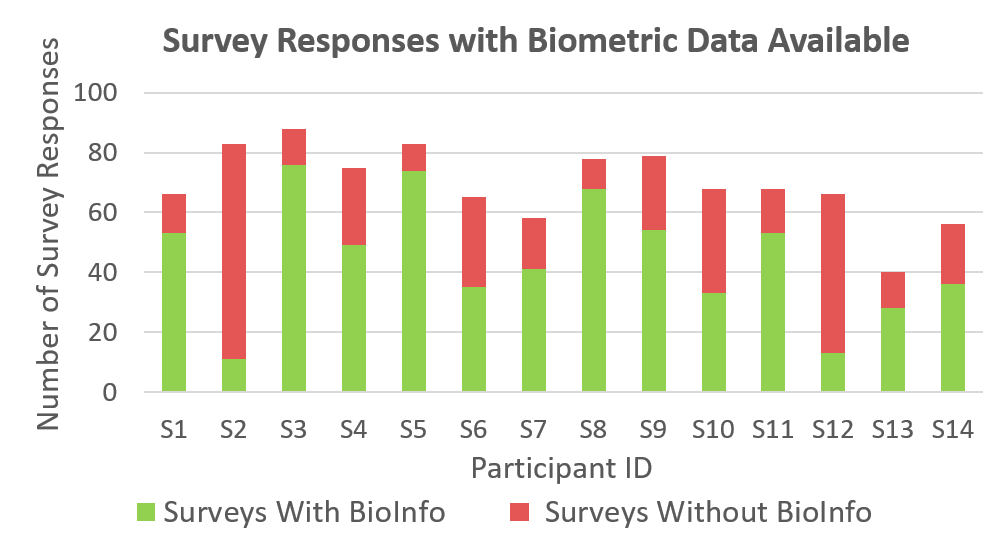
\includegraphics[width=0.5\textwidth]{DuringTheDay.png}
  \caption{The figure shows the biometric data available per each participant. Green sections represent survey responses with biometric
  data available, red sections responses with no biometric data available}
   \label{surveyBio}
   \vspace*{-4mm}
\end{figure}


\subsubsection{Feature Extraction}
We extracted features from the biometric data to provide as input to machine 
learning models. Previous 
studies~ \cite{vorburger05,zuger2015interruptibility} identify time windows as an 
important factor that impacts the prediction accuracy of a classifier. We 
considered many time windows from the literature on biometric 
analysis~\cite{zuger18}, ranging from 10 seconds to 3 hours. Specifically, we 
considered the following time windows: \textit{10sec, 20sec, 30sec, 45sec, 
1min, 2min, 3min, 5min, 7.5min, 10min, 20min, 30min, 45min, 1hour, 2hour, 
3hour}.

From the start time of each survey response, we look back the amount of time 
that corresponds to each time window, and we create features for all of the 
biometric data available in that time window. For example, if a participant 
started a survey response at 11:05am, for the 30min time window, we create 
features using all of the available biometric data from 10:35am to 11:05am. 
For each time window, we calculate 10 statistical measurements from the 
biometric data to create 10 distinct features. Specifically, the 10 
statistical measurements are: mean, standard deviation, variance, median, 
percentile25, percentile75, interquartile range, maximum, minimum, and 
range. Thus, for each survey response, we generate a large number of 
corresponding features based on three factors: biometric measurement, time 
window, and statistical measurement. In addition to these biometric 
features, we also considered the time of day in which the questions were 
asked. These features are created to predict the responses described by the 
ground truth.

\subsubsection{Response Transformations}
Table~\ref{responseDistribution} illustrates the distribution of responses from each participant for each of the three survey questions (listed in Section~\ref{sec:Surveys}). The figure shows that there is a notable imbalance in the distribution of the self-reported responses provided by the participants. Most participants did not use all five points of the five-point Likert scale in their responses, and the distributions tend to skew toward one side or the other, depending on the question. Thus, we binarized the survey data into a two-point scale to give the machine learning models the best possible chance to make useful predictions. The two points in the binary scale represent negative or positive responses for each of the three human aspects of interests (e.g., not stressed or stressed). 

We binarized the survey responses as follows. For each participant, we calculated the median response value for each question. We classified each response below the median as 0 ('negative') and each response above the median as 1 ('positive'). The distribution for the stress question skewed left, so we included the median values in the 'positive' class, while the distributions for focus and awakeness skewed right, so we included those median values in the 'negative' class.

\subsubsection{Oversampling}
Even after binarizing the responses as described in the previous section, we found the distribution of responses was still quite imbalanced for many of our participants. This can be seen in the distribution columns in Table \ref{tab:accuracy}. To combat this, we applied random oversampling to our training sets, which artificially rebalances the dataset by creating randomly replicated data in the minority class. This has been a commonly used technique in previous studies on unbalanced datasets \cite{chawla2004,yap2014}.


\begin{table}
  \centering
      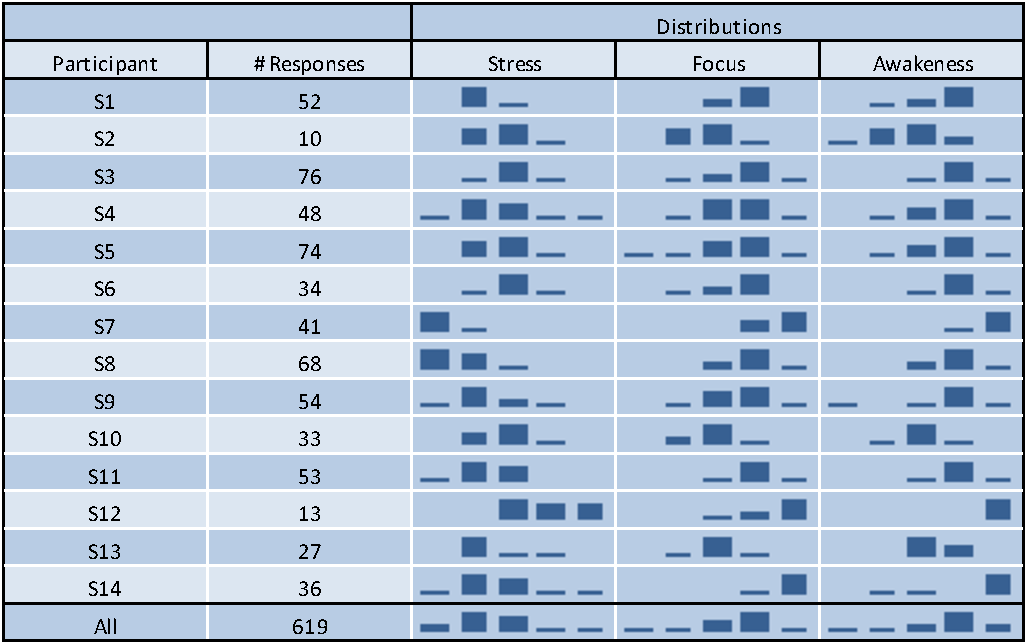
\includegraphics[width=0.5\textwidth]{distributiontable.pdf}
  \caption{The distribution of the responses of each participant to the three questions asked during the day are shown. Each bar in the histograms represent one of the 5 values on the 5-point Likert scale we asked participants to respond with, where the far left side of the histograms are 1/Not at all, and the far right sides are 5/Extremely}
   \label{responseDistribution}
   \vspace*{-2mm}
\end{table}


\subsection{Selecting a Classifier Algorithm}

There are many different algorithms that can be used to build a classifier. To select an
algorithm, we compared multiple classifiers using the popular machine learning library scikit-learn~\cite{pedregosa11} and performed a grid search analysis to determine the optimal hyperparameters for each classifier. Our analysis showed that random forest outperforms all other classifiers, including Na\"ive Bayes, decision trees, support vector machine, and a multilayer perceptron neural network. The optimal values for random forest and the three output measures are listed in Table \ref{tab:hyperparams}. For the remainder of this paper, we refer to random forest classifiers trained with these hyperparameters.%\\[-0.1cm]
% for stress they were (minimum samples for split = 4, # of estimators = 100, max features = 0.5, k=300), for focus they were (minimum samples for split = 4, # of estimators = 50, max features = 0.5, k=200), and for awakeness they were (minimum samples for split = 4, # of estimators = 100, max features = 0.25, k=800)
\begin{table}[h]
	\begin{centering}
	\small\addtolength{\tabcolsep}{-1pt}
    \begin{tabular}{llll}
      \hline
      Variable & K & \# Estimators & Minimum Samples Split \\
      \hline
      Stress & 300 & 100 & 4\\
      Focus & 200 & 50 & 4\\
      Awakeness & 800 & 100 & 4\\
      \hline
    \end{tabular}
    \caption{The hyperparameters selected by grid search analysis to tune our random forest models. K refers to the number of features selected.}    \label{tab:hyperparams}
    \end{centering}
\end{table}

\subsection{Individual Classifiers}
%\noindent\textit{Results of Individual Classifiers}\\
Since peoples' experience of stress, focus, and awakeness (as well as
their physiological manifestations) can vary substantially
(e.g.,~\cite{Hernandez11}), we first trained individual classifiers
for each participant (rather than a general one for all
participants). The results of our analysis are reported in
Table~\ref{tab:accuracy}. For our analysis, we report values of
accuracy, one of the most commonly used metric to compare performance,
as well as precision and recall of the classes of interest:
'stressed', 'not focused', and 'not awake'. Since the imbalance in the
data can lead to high accuracy values if a classifier always just
predicts the most likely/frequent class while ignoring the class of
higher importance and interest, precision and recall of the class of
interest are also important to
consider~\cite{yap2014,bhattacharyya_data_2011,Hernandez11}.

% However, the imbalance in the data can lead to a classifier with high accuracy if it always just predicts the more likely class while ignoring the class of higher importance and interest in our case (i.e. stressed, not focused, not awake). Therefore, we further report the precision and recall for the three classes 'stressed', 'not focused' and 'not awake'. 


Overall, we were able to use extracted physiological features to
predict all three aspects with reasonable accuracy, precision, and
recall, as well as to improve upon the baseline---a stratified random
classifier that randomly chooses one of the two classes with a bias
towards the larger class. While the individually trained classifiers
improved on average across all participants upon the baseline in all
cases excepting recall of 'not focused', the improvement was
substantially higher for awakeness (85\% improvement in precision,
62\% in recall, and 7\% in accuracy) than for stress or focus. Also,
the performance of the individually trained classifiers varied greatly
across participants. While some participants showed a large
improvement, for others the baseline performed much better than the
individually trained classifier. For instance, for predicting
'stressed', the individual classifiers improved upon the baseline for
S4, S6, S8, S11, S12, and S14 with a maximum improvement of 88.4\% in
precision and 184.6\% in recall for S12, while they did worse for S1,
S3, S5, S7, S9, S10, and S13, and in the worst cases did not correctly
predict a single instance of 'stressed'. Typically users that have the
lowest precision and recall values are those where the data is the
most unbalanced. This translates to a scenario where the classifier
will likely label the minority instances as part of the majority class
due to the unbalanced ratio of the data.\\[-0.1cm]
% We attribute these discrepancies to the large differences in response distributions between participants, as well as to the subjectivity of self-reporting.
%
%(improvement: 8\% precision, 1\% recall, 8\% accuracy), the individual performance varied greatly among participants. Some participants showed negligible difference in comparison to the baseline classifier, e.g. subject ..., while others showed a large improvement, e.g. subject ...
%\begin{table}[h!]
%\begin{centering}
%\begin{tabular}{lll}
%\hline
%Participant & Recall Improvement (\%) & Precision Improvement (\%)\\
%\hline
%S12 & 184.6 & 88.4 \\
%S6 & 66.7 & 85.8 \\
%S11 & 50.0 & 44.4 \\
%S8 & 32.4 & 26.7 \\
%S14 & 14.7 & 9.8 \\
%S4 & 5.6 & 5.5 \\
%S9 & -55.4 & -46.8 \\
%S3 & -90.0 & -82.1 \\
%S1 & -100.0 & -100.0 \\
%S5 & -100.0 & -100.0 \\
%S7 & -100.0 & -100.0 \\
%S10 & -100.0 & -100.0 \\
%S13 & -100.0 & -100.0\\
%S2 & - & -\\
%\hline
%\end{tabular}
%\caption{Percentage improvement in recall and precision for stress, using our approach compared to the baseline, on an individual level. For participant 2, the baseline achieved a precision and recall of 0, thus the improvement is undefined}
%\end{centering}
%\label{tab:indImprovement}
%\end{table}


\subsection{Feature Selection and Importance}
%\noindent\textit{Feature Selection and Importance}\\
There are a large variety of features that can be (and have been) calculated in previous research for each of the basic measurements listed in Table~\ref{signals}, such as the mean, standard deviation, maximum, and interquartile range. In addition, each of these metrics can be combined with the various time windows captured of a basic measurement, resulting in a large feature space. To reduce the feature space, we experimented with multiple feature selection methods, including selecting the top k highest correlated features by various metrics such as mutual information, Pearson's correlation coefficient, ANOVA's F-value, as well as wrapper methods such as recursive feature elimination, optimizing mean decrease accuracy by iteratively permuting features, and only selecting features that exceed a certain Gini importance threshold. We found that all methods produced similar results with respect to accuracy, precision, and recall for the individual models. Ultimately, we chose to use the top k features with the highest ANOVA F-value, as it is relatively simple and efficient to calculate. The values of k used were selected by grid search analysis, and are shown in Table \ref{tab:hyperparams}. 

%Respiration rate is also highly important for stress (#3 , 14.4%) but I'm not sure what previous works say about correlation with stress
Overall, the features that were selected as the important ones for the individual models based on the random forest algorithm varied greatly across participants. Yet, some feature categories were considered to be important more frequently than others. Table~\ref{tab:featureImportance} shows the averaged Gini importance for the feature categories used for predicting stress. Particularly important for stress were the feature categories heart rate variability (18.3\%) and skin temperature (15.7\%), both of which have been shown in several previous studies to be  indicators for stress~\cite{dishman2000stress,mcduff16,kataoka00}. For predicting focus, the feature categories for blood pulse wave (14.2\%) and heart rate variability (13\%) showed to be the most important categories, while for awakeness the most important ones were heart rate variability (13.6\%) and blood pulse wave (13.1\%).\\[-0.1cm]


\begin{table}[h!]
  \begin{centering}
  \begin{tabular}{llll}
    \hline
    Feature Category & Stress & Focus & Awakeness\\
    \hline
    Heart Rate Variability & 18.3\% & 13\% & 13.6\%\\
    Blood Pulse Wave & 10\% & 14.2\% & 13.1\%\\
    Heart Rate & 8.7\% & 12.6\% & 10.3\%\\
    Skin Temperature & 15.7\% & 9.8\% & 10\%\\
    Galvanic Skin Response & 6.6\% & 8.2\% & 5.1\%\\
    Respiration Rate & 14.8\% & 12.7\% & 10\%\\
    Oxygen Saturation & 5.6\% & 4.3\% & 2\%\\ 
    Energy Expenditure & 6\% & 7.7\% & 4.8\%\\
    Activity & 4.6\% & 7.8\% & 7.6\%\\
    Steps & 1.7\% & 0.8\% & 0.9\%\\
    Time of Day & 0\% & 0.1\% & 0.5\%\\
    \hline
  \end{tabular}
  \caption{The averaged Gini importance of each feature category, per response variable.}
  \label{tab:featureImportance}
  \end{centering}
  \vspace*{-2mm}
\end{table}

\subsection{Individual vs.\ General Model}
%\noindent\textit{Individual vs.\ General Model}\\
Individual models are trained specifically for each individual and thus require a data collection period before they are capable of making accurate predictions. On the other hand, the idea of general models is to be able to train them on already collected data and then  to be able to apply them even to new and unseen individuals, thus overcoming the cold-start problem. Given the large individual differences in biometrics, training a general model to achieve an adequate accuracy for new individuals is not necessarily possible. 

To examine the performance of a general model for our participants, we trained three general models, one for focus, one for awakeness and one for stress. We roughly followed the same procedure as for the individual models. Due to the larger amount of data available in the general case, we used the more common random undersampling, which randomly selects elements in the majority class to exclude from the dataset, instead of random oversampling to balance the distribution of the dataset. The models were trained on the datasets of 13 of the 14 participants, and then evaluated on the dataset of the last, repeating this process for all 14 participants. 

The bottom row of Table \ref{tab:accuracy} presents the averaged performance results for this approach in terms of accuracy, precision, and recall. Although the averaged precision and recall are comparable or better than those of the averaged individual results, this was at the cost of a large decrease in overall accuracy. Upon closer investigation into the performance of the general model when testing on each participant, we found that individually trained models for each participant performed much better than a general model trained over all participants. Using stress as an example, for participant S12, for whom we saw the greatest increase compared to the baseline in individual models, the general model was unable to predict a single instance of 'stressed' correctly. This is consistent with our expectations because biometric features are highly specific to individuals.


%\todo{put the content of the following sentence somewhere into the discussion; We attribute these discrepancies to the large differences in response distributions between participants, as well as to the subjectivity of self-reporting.}

